\documentclass[natbib]{sigplanconf}

% \usepackage{dingbat}
\usepackage{pifont}
\usepackage{booktabs}
\usepackage[usenames,dvipsnames]{color}
\usepackage{mathptmx}
\usepackage[scaled=.92]{helvet} % see www.ctan.org/get/macros/latex/required/psnfss/psnfss2e.pdf
\usepackage{graphicx}
\usepackage{xspace}
\usepackage{listings}
\lstset{language=Java,basicstyle=\small\sffamily,columns=flexible,numberstyle=\em\scriptsize,frame=none,mathescape=true,escapeinside={/**}{*/}}
\newcommand{\code}[1]{\lstinline|#1|\xspace}
\newcommand{\javac}{javac\xspace} % This package lets you punctuate \javac normally and get good spacing, e.g., \javac.  gives you: javac.
\usepackage{url}  % particularly useful for URLs in bib entries
% packages
\usepackage{slashed}

\usepackage{array}
\usepackage{longtable}
\usepackage{amsmath}
\usepackage{amssymb}
\usepackage{amsthm}


\usepackage{stmaryrd}
\usepackage{ifthen}
\usepackage{marvosym}
\usepackage{graphicx}
\usepackage{calc}
\usepackage{wasysym}
\usepackage{rotating}

% \usepackage{pdfsync}
% \usepackage{proof}
% \usepackage{bussproofs}
% \usepackage{mathpartir}
% \usepackage{varwidth}

% \usepackage{tikz}
% \usetikzlibrary{calc}
% \usetikzlibrary{arrows}
% \usetikzlibrary{positioning}
% \usetikzlibrary{chains}
% \usetikzlibrary{decorations.pathmorphing}
% \usetikzlibrary{decorations.pathreplacing}
% \usetikzlibrary{shapes.misc}
% \usetikzlibrary{shapes.multipart}
% \usetikzlibrary{shapes.geometric}
% \usetikzlibrary{backgrounds}

% Select symbols from bbding
\newcommand{\dingfamily}{\fontencoding{U}\fontfamily{ding}\selectfont}
\newcommand{\dingSymbol}[1]{{\dingfamily\symbol{#1}}}
\newcommand{\RectangleThin}{\dingSymbol{'164}}
\newcommand{\Rectangle}{\dingSymbol{'165}}
\newcommand{\RectangleBold}{\dingSymbol{'166}}

% semantic styles
% \usepackage[ligature,shorthand,reserved]{semantic}
% \newcommand{\semanticdomainstyle}[1]{%
%   \ensuremath{\mathchoice%
%     {\mbox{\textit{#1}}}%
%     {\mbox{\textit{#1}}}%
%     {\mbox{\textit{\scriptsize#1}}}%
%     {\mbox{\textit{\tiny#1}}}}}
% \reservestyle{\semanticdomain}{\semanticdomainstyle}
% \semanticdomain{Int[\ensuremath{\mathbb{Z}}]}

% \newcommand{\semanticvaluestyle}[1]{\ensuremath{\bf{\mathrm{#1}}}}
% \reservestyle{\semanticvalue}{\semanticvaluestyle}

% Rotating characters
\newcommand{\rotxc}[1]{\begin{sideways}#1\end{sideways}}
\newcommand{\rotrotxc}[1]{\rotxc{\rotxc{#1}}}


% Funky underline types
\def\dotuline{\bgroup
  \ifdim\ULdepth=\maxdimen  % Set depth based on font, if not set already
   \settodepth\ULdepth{(j}\advance\ULdepth.4pt\fi
  \markoverwith{\begingroup
  \advance\ULdepth0.08ex
  \lower\ULdepth\hbox{\kern.15em .\kern.1em}%
  \endgroup}\ULon}

\def\dashuline{\bgroup
  \ifdim\ULdepth=\maxdimen  % Set depth based on font, if not set already
   \settodepth\ULdepth{(j}\advance\ULdepth.4pt\fi
  \markoverwith{\kern.15em
  \vtop{\kern\ULdepth \hrule width .1em}%
  \kern.01em}\ULon}

% Common constructs
\renewcommand{\iff}{\text{ iff }}
\newcommand{\hole}{\Box}
\newcommand{\true}{\mathsf{true}}
\newcommand{\fail}{\mathsf{fail}}
\newcommand{\false}{\mathsf{false}}
\newcommand{\strue}{\mathrm{T}}
\newcommand{\sfalse}{\mathrm{F}}

% math ligatures
% \mathlig{--`}{\rightharpoonup} % partial function
% \mathlig{|->}{\mapsto} % tight points-to
% \mathlig{->}{\rightarrow} % remap for functions
% \mathlig{-->}{\longrightarrow} % remap for functions
% \mathlig{[[}{\llbracket} % open double bracket
% \mathlig{]]}{\rrbracket} % close double bracket
% \mathlig{<=>}{\Leftrightarrow}

% quantifiers
\newcommand{\A}[1][]{\forall \ifthenelse{\equal{#1}{}}{}{\mbox{$#1.$}\ }}
\newcommand{\E}[1][]{\exists \ifthenelse{\equal{#1}{}}{}{\mbox{$#1.$}\ }}
\newcommand{\Lam}[1][]{\lambda \ifthenelse{\equal{#1}{}}{}{\mbox{$#1.$}\ }}
\newcommand{\Am}[1][]{\forall_{\!*} \ifthenelse{\equal{#1}{}}{}{#1.\,}}
\newcommand{\Em}[1][]{\exists_{*} \ifthenelse{\equal{#1}{}}{}{#1.\,}}
\newcommand{\nA}[1][]{\not\forall \ifthenelse{\equal{#1}{}}{}{#1.\,}}
\newcommand{\nE}[1][]{\nexists \ifthenelse{\equal{#1}{}}{}{#1.\,}}

% Common functions
\newcommand{\dom}{\mathit{dom}}

% Common Decorations
\newcommand{\defemph}[1]{\textbf{#1}}
\newcommand{\estate}[1]{\langle #1 \rangle}

% make eqnarrays have more space
\renewcommand\arraystretch{1.2}

% Theorem Environments
\newtheorem{lem}{Lemma}
\newtheorem*{lemstar}{Lemma}
\newtheorem{thm}{Theorem}
\newtheorem{corr}{Corollary}
\newtheorem{defn}{Definition}
\newtheorem{claim}{Claim}
\newtheorem{obs}{Observation}
\newtheorem{prob}{Problem}

% comment blocks
\newcommand{\deleted}[1]{}
\newcommand{\draftonly}[1]{}
\newcommand{\stephencomment}[1]{
\begin{quote}
{\bf *** Stephen says:} {\it #1}
{\bf ***}
\end{quote}}

% indentation
\newcommand{\ind}{\hspace*{0.5cm}}

% \usepackage[ruled]{algorithm2e}
% Algorithm package options
% \SetInd{1ex}{1ex}

% extra algorithm constructs
% \SetKwIf{Let}{Failed}{let}{in}{match failed $=>$}{end}
% \SetKwSwitch{Match}{MCase}{MOther}{match}{with}{}{\_}{end}
% \SetKwInput{Type}{Type}
% \SetKwBlock{Ind}{\vspace{-3ex}}{}
% \SetKwBlock{IndEnd}{\vspace{-3ex}}{end}
% \SetKwIf{DefFn}{}{fun}{=}{}{in}
% \SetKwFor{uForEach}{foreach}{do}{\vspace{-3ex}}

\newcommand{\none}{\mathsf{None}}
\newcommand{\some}[1]{\mathsf{Some}\bigl(#1\bigr)}
\newcommand{\somenop}[1]{\mathsf{Some}#1}

% Bnf definitions
\newcommand{\GoesTo}{\mathrel{::=}}
\newcommand{\bnfdef}{\GoesTo}
\newcommand{\bnfalt}{\Or}
\newcommand{\bnfas}{\bnfdef}

% Math constructs
\newcommand{\sembrack}[1]{\llbracket#1\rrbracket\,}
\newcommand{\imp}{=>}

% Transition systems
\newcommand{\steps}[1]{\stackrel{#1}{\rightarrow}}
\newcommand{\stepst}[1]{\stackrel{#1}{\rightarrow^{*}}}
\newcommand{\stepsp}[1]{\stackrel{#1}{\rightarrow^{+}}}
\newcommand{\gentrans}{\dashrightarrow}
\newcommand{\gentransnum}[1]{\stackrel{#1}{\dashrightarrow}}
\newcommand{\trans}[1][]{\stackrel{#1}{\leadsto}}
\newcommand{\transt}[1][]{\mathrel{\trans[#1]{\!\!}^{*}}}
\newcommand{\transp}[1][]{\mathrel{\trans[#1]{\!\!}^{+}}}

%% derivation rules
% note that horizontal space can be hacked with:
%% \def \mpr@andskip {1em plus 0.25fil minus 0.25em}
% \renewcommand{\TirName}[1]{$#1$}
% \renewcommand{\RefTirName}[1]{$#1$}

\newcommand{\infrulelabel}[1]{\mbox{\normalfont\small\textsc{#1}}}
\newcommand{\drule}[4][]
  {\inferrule*[lab=\<#2>,right=\ensuremath{#1}]{#3}{\textstyle#4}}
\newlength{\templength}
\newcommand{\userule}[4][leftskip=0em]
  {\inferrule*[right=\textsc{#2},before=\setlength{\templength}{\widthof{\textsc{#2}}},rightskip=\templength,#1]{#3}{\textstyle#4}}
\newcommand{\daxiom}[3][]{\drule[#1]{#2}{ }{#3}} % derivation axiom
\newcommand{\daxiombc}[3]{\drulebc{#1}{#2}{ }{#3}}
\newcommand{\usingrule}[3]{\prooftree[#1]\using#2\leadsto#3\endprooftree}
\newcommand{\belowcondition}[1]{\rule{0pt}{3ex} {}^\dagger #1}
\newcommand{\drulebc}[4]{\drule[{}^\dagger]{#2}{#3}{#4\\\\\belowcondition{#1}}}
\newcommand{\eqjudg}[2]{\stackrel{\textstyle#1}{#2}}
%% \newcommand{\eqjudg}[2]{\begin{eqnalign}[c][b]#1\\[-2.5ex]#2\end{eqnalign}}
\newcommand{\pfdots}[1]{\stackrel{\textstyle\vdots}{#1}}

% \reservestyle{\infrule}{\infrulelabel}
% \infrule{}

% Stacking
\newcommand{\stacklabel}[1]{\stackrel{\smash{\scriptscriptstyle \mathrm{#1}}}}
\newcommand{\Def}{\stacklabel{def}}
\newcommand{\Fin}{\stacklabel{fin}}

\newcommand{\spec}[3]{\{#1\}\;#2\;\{#3\}} % Hoare triple

% Separation Logic
\newcommand{\emp}{\mathbf{emp}}
\newcommand{\pto}{\mapsto}
\newcommand{\lbl}[1]{\mathsf{#1}}
\newcommand{\dll}[1]{\mathrm{dll}(#1)}

% Program commands
\newcommand{\assume}{\mathsf{assume}}
\newcommand{\nondet}[1]{#1 :=\ ?}


\newcommand{\TOSAcronym}{\emph{Targeted Object Synthesis} (TOS)\xspace} 
\newcommand{\TOS}{TOS\xspace} 

\newcommand{\stephen}[1]{\textcolor{Red}{Stephen: #1}}
\newcommand{\sbm}[1]{\textcolor{Red}{Stephen: #1}}
\newcommand{\suriya}[1]{\textcolor{blue}{Suriya: #1}}
\newcommand{\kathryn}[1]{\textcolor{blue}{Kathryn: #1}}
\newcommand{\mwh}[1]{\textcolor{blue}{Mike: #1}}
\newcommand{\todo}[1]{\textcolor{red}{#1}}

\begin{document}

\conferenceinfo{Mystery'12,} {Rome, Italy.}
\CopyrightYear{2012}
\copyrightdata{2012}


\title{Automating Object Transformations for Dynamic Software Updating
%   \thanks{COMMENT OUT FOR SUBMISSION, UNCOMMENT FOR final version. Some of these may or may not apply to your work.  Make Kathryn check.
%     This work is supported by NSF SHF-0910818, NSF CSR-0917191, NSF
%     CCF-0811524, NSF CNS-0719966, NSF CCF-0429859, Intel, IBM, CISCO,
%     Google, and Microsoft.  Any opinions, findings and conclusions
%     expressed herein are the authors' and do not necessarily reflect
%     those of the sponsors.}
    }

% 2008: NSF EIA-0303609, DARPA F33615-03-C-4106,


\authorinfo{Anonymous}{}{}
%% \authorinfo{Stephen Magill, Michael Hicks}
%%            {University of Maryland, College Park}
%%            {smagill@cs.umd.edu}

%% \authorinfo{Suriya Subramanian}
%%            {Intel Corporation}
%%            {suriya@gmail.com}

%% \authorinfo{Kathryn S. McKinley}
%%            {Microsoft Research}
%%            {mckinley@cs.utexas.edu}

\maketitle

\begin{abstract}
  Dynamic software updating (DSU) systems eliminate costly downtime by
  dynamically fixing bugs and adding features to executing programs.
  Given a static \emph{code} patch, most DSU systems can construct the
  run-time code changes automatically.  However, a dynamic update must
  also specify how to change the running program's execution
  \emph{state}, e.g., its stack and heap, to be compatible with the
  new code.  Constructing such \emph{state transformations} correctly
  and automatically remains an open problem.  This paper presents a
  solution called \TOSAcronym.  \TOS first executes the same tests on
  the old and new program versions separately, observing the program
  state at key points.  Given two corresponding states, \TOS
  \emph{matches} corresponding objects between the two versions, and
  \emph{synthesizes} the simplest-possible function to transform old
  version objects to their corresponding new versions.  We show the
  efficacy of \TOS by inferring transformation functions for actual
  updates to four open-source server programs.
\end{abstract}


% {\scriptsize
% \category{D.3.4}{Programming Languages}{Processors}[Memory management (garbage collection); Optimization] 
% \terms
% Experimentation, Languages, Performance, Measurement
% \keywords
% Heap
% }

\newcommand{\eqf}[1]{=_{#1}}
\newcommand{\eqfv}[2]{=_{#1:#2}}
\newcommand{\eqfvclass}[2]{[#2]_{#1}}
\newcommand{\eqfclass}[2]{[#2]_{#1}}
\newcommand{\fset}{F}
\newcommand{\objset}{O}
\newcommand{\setsize}[1]{\lvert #1 \rvert}
\newcommand{\no}{\hat{o}}
\newcommand{\nobjset}{\hat{O}}
\newcommand{\nL}{\hat{L}}

\newcommand{\se}{\textit{se}}
\newcommand{\oldvar}{\textrm{o}}
\newcommand{\newvar}{\textrm{n}}
\newcommand{\casestart}{\textsf{case }}
\newcommand{\caseend}{\textsf{ end}}
\newcommand{\carrow}{\Rightarrow}
\newcommand{\sconcat}{\textsf{concat}}
\newcommand{\filtermap}{\textsf{filtermap}}
\newcommand{\map}{\textsf{map}}
\newcommand{\delim}{\textit{delim}}
\newcommand{\substr}{\textsf{substr}}
\newcommand{\op}{\mathrel{\diamond}}

\newcommand{\degree}[2]{\textit{degree}_{#1}(#2)}
\newcommand{\maxdegree}[1]{\textit{degree}_\textrm{max}(#1)}
\newcommand{\atrace}{\alpha}
\newcommand{\env}{\epsilon}
\newcommand{\runprog}[3]{\textit{runprog}(#1,#2,#3)}
\newcommand{\values}[2]{\textit{values}_{#1}(#2)}
\newcommand{\set}{\sigma}
\newcommand{\setlst}{\vec{\set}}
\newcommand{\concat}{\mathrel{\textit{::}}}
\newcommand{\restrictval}[3]{#1 \mathord\downharpoonright_{#2 = #3}}
\newcommand{\lstlength}[1]{\textit{length}(#1)}
\newcommand{\equivcount}{\stackrel{\#}{=}}
\newcommand{\updset}{\Delta}
\newcommand{\matching}[1]{\sim_{#1}}
\newcommand{\return}{\textbf{ret}}

\newcommand{\inset}{\sigma_{\text{in}}}
\newcommand{\outset}{\sigma_{\text{out}}}
\newcommand{\rank}[3]{\mathit{rank}(#1,#2,#3)}
\newcommand{\anew}[1]{\mathsf{new}\ #1}

\newcommand{\slold}{\setlst_{\mathit{old}}}
\newcommand{\slnew}{\setlst_{\mathit{new}}}


% \stephencomment{K; Fixed. TODO: unify notation.  We are currently using $o$ and $n$ in some places for old/new object, whereas in others we use $o$ and $o'$.  Also $o_1$ and $o_2$ pop up sometimes.}
\section{Introduction}

Suppose you are running an on-line service and a memory leak in your
server software causes it to regularly run out of memory and
crash.  Eventually you discover the one-line fix: the
\code{Connection} class's \code{close} method should
unlink some metadata when a connection closes.  To apply this
fix in a standard deployment you stop your server and restart
the patched version, but in doing so disrupt any active users.  With 
\emph{dynamic software updating} (DSU) support in an extended Virtual Machine
such as LiveRebel~\cite{javarebel} you
can do better. You apply a \emph{dynamic} patch 
to the \code{Connection} class of your \emph{running}
system to prevent further leaks without disrupting current users.
In some DSU-enhanced VMs, such as Jvolve~\cite{jvolve}, you can do better
still. You include \emph{state 
  transformation} code in your dynamic patch that traverses the
heap and unlinks the useless metadata left reachable by the bug.

% Prior work shows how to implement code and
% data updates with special compilation support~\cite{update-streaks},
% run-time binary rewriting~\cite{}, and extended virtual machine (VM)
% functionality~\cite{jvolve}.    They further demonstrate successful
% application of years' worth of changes to applications and servers,
% such as the OpenSSH daemon, Very Secure FTP daemon (vsftpd), and
% memcached, to running systems to bring them up to date, even when they
% are actively performing work~\cite{jvolve,update-streaks}.

An important goal toward furthering the adoption of DSU systems is to
make them easy to use, i.e., to minimize the effort required to
produce a correct dynamic patch from two versions of a system.  As a
step in this direction, many DSU systems employ simple
\emph{syntactic}, \emph{type-based} tool support for constructing a
dynamic patch from the old and new program
versions~\cite{jvolve,ksplice,neamtiu06dsu, HicksNettles03}.  For
example, if class \code{C}'s method \code{m}'s bytecode has changed, Jvolve
will include \code{C.m} in the dynamic patch.  If \code{C}'s field
definitions change, in type or number, Jvolve creates a default
\emph{object transformation function} that it  applies to all
\code{C} objects when it applies the patch. This function retains
the values of unchanged fields and initializes the rest with a default
value, e.g., \code{null}.

While tool support for identifying changed code is highly effective,
existing support for constructing state transformation code is rarely
sufficient, and the programmer must therefore modify the generated code.  
For example, in Jvolve the programmer must  add code that
unlinks the leaked metadata in our example.  Unfortunately, the cases
that require manual intervention are often challenging to get right.
For our example, the \code{Connection} transformer cannot simply unlink all
connection metadata unconditionally. Instead, it must use appropriate
context by examining the running program's heap and stack to
identify and unlink only the metadata that is logically dead.
Transformations that require moving objects between collections or
partitioning single objects into several objects---examples we have
observed in practice---require similar care in their construction.
Thus, writing state transformation code for DSU systems is a  programming task unique to DSU, and it can be
a time-consuming, error-prone process.

This paper presents a
general-purpose approach for synthesizing object transformers for
dynamic patches, to ease the burden on programmers.  Our \emph{Targeted Object
  Synthesis} (\TOS) approach was developed for the Java-based DSU system Jvolve, but
our techniques should adapt readily to other DSU systems that support state
transformation.

% shows how to automatically synthesize object state
% transformers and thus in many cases, significantly reduce or eliminate
% developer effort due to DSU.  

\TOS works in two phases, \emph{matching} and \emph{synthesis}.  The
matching phase begins by running both versions of the program on the
same inputs and taking heap snapshots at corresponding program points.
Given a class \code{C} for which to synthesize a transformer function
(i.e., because the class changed between versions), the goal is to
find corresponding \code{C} objects in each pair of corresponding
snapshots.  \TOS matching first attempts to match objects according to
\emph{key fields}, which are fields in an object that (1) uniquely
identify the object in a given heap (i.e., each object of class
\code{C} differs on the values of its key fields) and (2) there exist
objects in both heaps with the same values for these fields.  We use a
greedy algorithm which, in our experience, very often succeeds in
finding a set of key fields.  In the case that no key fields exist,
matching uses the most distinguishing set of fields it can find to
pair up most of the objects, and then applies a lightweight form of
synthesis (described next) to find a function that pairs up objects
that remain.

With pairs of corresponding objects $(o,o')$ in hand, \TOS
\emph{synthesis} searches for functions that are consistent with the
examples, i.e., functions $\delta$ for which $\delta(o) = o'$ for all
matched pairs.  Functions $\delta$ assign an expression to each
new-version object field one at a time, where the expressions may
reference any of the old object's fields (or fields reachable from
them).  These expressions may also contain constants, simple functions
(e.g., the concatenation or partitioning of string expressions), and
conditionals (e.g., if the value to assign to a field depends on the
current value of another field).  For fields that are collections, we
recursively invoke synthesis on the objects that make up each
collection, mapping the resulting function over the old collection
objects to produce the new one.  When many functions are possible for
a given set of examples, synthesis chooses the simplest.  The language
for expressing transformation functions $\delta$ was carefully chosen so that
important operations (like intersecting a set of candidate functions)
are efficient, while still being expressive enough to handle real
examples.


As far as we are aware, no prior work attempts \TOS matching, i.e.,
mapping heap objects from different program version executions.  The
\TOS synthesis step is similar to recent work on synthesizing string
and Excel table data transformation functions from input and output
examples~\cite{Gulwani:popl:2011,Gulwani:pldi:2011}.  \TOS matching
creates examples \emph{automatically}, whereas the prior work requires
users to provide examples.  \TOS functions are a superset of string
transformations. Excel table functions focus on filters and numerics,
where as \TOS data transformations focus on objects, and furthermore,
\TOS generates the examples from unstructured heap snapshots.

% \TOS is similar to recent work on
% synthesizing string, Excel table, and code transformation functions
% from input and output
% examples~\cite{Gulwani:popl:2011,Gulwani:pldi:2011,MKM:11}.  Whereas
% this work requires users to specify the examples, \TOS generates
% them. \TOS also requires a richer
% transformation domain than prior work.  For example, object
% transformers are a superset of string transformations, and more
% general than table or code insertion and deletion functions.

We demonstrate our approach by synthesizing transformation functions
for updates to several open-source Java servers, including
JavaEmailServer (a POP and SMTP server), CrossFTP (an FTP server),
Azureus (a Bittorrent client), and JEdit (a graphical text
editor). We show that \TOS
produces correct transformation functions for a variety of actual program
updates, whose changes require transformers that handle object field
additions, string partitioning, partitioning a collection based on a
predicate, and deleting objects due to memory leaks.  In fact, to our
knowledge no prior evaluation of a DSU system has considered the need
to correct the residual effects of a memory leak, and our synthesized
functions are the first demonstration of this capability.

In summary, this paper's contribution is \emph{Targeted Object
  Synthesis}, a method for automatically generating data
transformation functions needed by dynamic patches, which we have
shown to be practical by considering a variety of real-world examples.

\section{Overview}
\label{sec:overview}

This section presents an overview of synthesizing state transformation
functions for dynamic software updates using \TOS.  We begin with some
background on DSU, present an example dynamic update taken from an
actual program change, and show how \TOS synthesizes this dynamic update
automatically.

\subsection{Dynamic software updating}

Suppose an old version of a program is actively running, and a new
version becomes available that fixes some bugs or adds some new
features.  Since the running program contains useful program state
(e.g., active connections), we would like to update it without
shutting it down.  To use a typical DSU system to do so, we must
construct a \emph{dynamic patch}~\cite{HicksNettles03} that specifies
the changed code and a \emph{state transformation function}, which
modifies heap objects and other program state, as necessary, to be
compatible with the new code.  For example, if the old program version
maintains a list of \code{Connection} objects and the new version adds
some fields to the \code{Connection} class, the state transformation
function must initialize the values of the new fields for the existing
objects.  In some systems, the state transformer may also update the
\emph{control state} of the program, e.g., examining and modifying the
existing stack and program counter as necessary~\cite{upstare,jvolve}.
Our \TOS design generalizes across DSU systems, and we implement \TOS
for Jvolve~\cite{jvolve}, which performs DSU in a Java Virtual
Machine (based on Jikes RVM).

\begin{figure}
%\begin{wrapfigure}[13]{r}{2.5cm}
\begin{center}
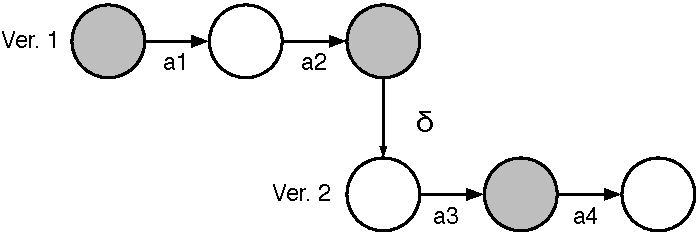
\includegraphics[scale=0.55]{updated-program-trace}
% \begin{tikzpicture}
% [circ/.style={draw,circle,minimum size=0.3cm},
%  label distance=0.1cm,
%  node distance=0.65cm]
% \node[circ,label=left:\small Ver. 1] (a1) {};
% \node[circ,right=of a1] (a2) {};
% \node[circ,right=of a2] (a3) {};
% \node[circ,below=of a3,label=left:\small Ver. 2] (b3) {};
% \node[circ,right=of b3] (b4) {};
% \node[circ,right=of b4] (b5) {};
% \path (a1) edge[->,auto,swap] node {\small $a_1$} (a2);
% \path (a2) edge[->,auto,swap] node {\small $a_2$} (a3);
% \path (a3) edge[->,auto] node {\small $\delta$} (b3);
% \path (b3) edge[->,auto,swap] node {\small $a_3$} (b4);
% \path (b4) edge[->,auto,swap] node {\small $a_4$} (b5);
% \end{tikzpicture}
\end{center}
\caption{\label{fig:hybrid}Trace of an updated program at update point
  after a2.}
%\end{wrapfigure}


%\begin{figure}
%\begin{wrapfigure}[13]{r}{2.5cm}
\begin{center}
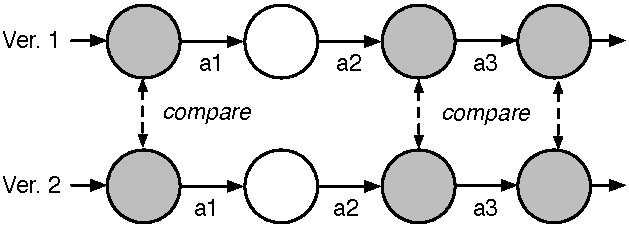
\includegraphics[scale=0.55]{comparing-heaps-two-runs}
% \begin{tikzpicture}
% [circ/.style={draw,circle,minimum size=0.3cm},
%  label distance=0.1cm,
%  node distance=0.65cm]
% \node[circ,label=left:\small Ver. 1] (a1) {};
% \node[circ,right=of a1] (a2) {};
% \node[circ,right=of a2] (a3) {};
% \node[circ,below=of a1,label=left:\small Ver. 2] (b3) {};
% \node[circ,right=of b3] (b4) {};
% \node[circ,right=of b4] (b5) {};
% \path (a1) edge[->,auto,swap] node {\small $a_1$} (a2);
% \path (a2) edge[->,auto,swap] node {\small $a_2$} (a3);
% \path (a3) edge[<->,densely dashed,auto] node {\small compare} (b5);
% \path (b3) edge[->,auto,swap] node {\small $a_1$} (b4);
% \path (b4) edge[->,auto,swap] node {\small $a_2$} (b5);
% \end{tikzpicture}
\end{center}
\caption{\label{fig:run-both}Comparing old \& new version heaps at update points.}
%\end{wrapfigure}
%\end{figure}
\end{figure}

Figure \ref{fig:hybrid} depicts a dynamically updated program's
execution.  The circles represent the program's state, the labels
$a_1, a_2, a_3, a_4$ represent \emph{actions}, e.g., messages sent to
and from client applications.  Each gray circle represents a state in
which a dynamic update is permitted by the system, if one is available
(discussed more below).  In this trace, the program starts executing
at version 1, and after executing actions $a_1$ and $a_2$, it applies
a dynamic patch.  As a result, the code of the program is updated to
version 2, and the state transformation function $\delta$ is applied
to transform the current state.  A patch could have been applied in
the initial state or the one after $a_3$, too, but no patch was
available.

\begin{figure*}[t]
\begin{tabular}{c|c|c}
\begin{minipage}{2.4in}
\begin{lstlisting}
public class User {
  private final String username, domain, password;
  private String[] forwardAddresses;
  public User(...) {...}
  public String[] getForwardedAddresses() {...}
  public void setForwardedAddresses(String[] f) 
  {...}
}
public class ConfigurationManager {
  private User loadUser(...) {
     ...
     User user = new User(...);
     String[] f = ...;
     user.setForwardedAddresses(f);
     return user;
  }
}
\end{lstlisting}
\end{minipage} &
\begin{minipage}{2.5in}
\begin{lstlisting}
public class User {
  private final String username, domain, password;
  private EmailAddress[] forwardAddresses;
  public User(...) {...}
  public EmailAddress[] getForwardedAddresses() {...}
  public void setForwardedAddresses(EmailAddress[] f) 
  {...}
}
public class ConfigurationManager {
  private User loadUser(...) {
     ...
     User user = new User(...);
     EmailAddress[] f = ...;
     user.setForwardedAddresses(f);
     return user;
  }
}
\end{lstlisting}
\end{minipage} &
\begin{minipage}{1.2in}
\begin{lstlisting}
public class EmailAddress {
  public EmailAddress(
    String username, 
    String domain
  ) {
    _isEmpty = false;
    _username = username;
    _domain = domain;
  }
  ...
  private String _username = "";
  private String _domain = "";
  private boolean _isEmpty = true;
}   
\end{lstlisting}
\end{minipage} \\
(a) Version 1.3.1 &
(b) Version 1.3.2 &
(c) Common code \\
\end{tabular}
\caption{An update to JavaEmailServer (JES) \code{User} and
  \code{ConfigurationManager} classes}
\label{fig:email-example}
\end{figure*}

Most DSU systems work in three steps.  First, they dynamically load
the new and changed code.  Second, they redirect existing references
to the new definitions.  Finally, they execute the state
transformation function to update the existing state.  Jvolve
implements these steps within a modified virutal machine. It uses
standard classloading to load new versions of classes.  For classes
whose only change is to the code of methods, Jvolve simply modifies
the metadata for that class to point to the new method definitions
(which the JIT may subsequently optimize).  For each class whose
objects' state requires modification (e.g., because the new version
adds fields), the patch must include an \emph{object transformation
  method}.  At update time, the garbage collector finds all objects
that require transformation. It executes the object transformation
method on each old object, creating a new corresponding object that
conforms to the new class's type specification and initializing its
state.

When a dynamic patch becomes available the system may choose not apply
it immediately.  A policy adopted by many DSU systems is to delay
updates while changed code is actually executing or referenced by the
call stack.  While this delay makes sense, it is not sufficient to
avoid trouble.  Hayden et al.~\cite{hayden11testing-journal} studied
several years' worth of changes to three server programs and found
that dynamic updates derived from actual releases sometimes fail even
while adhering to this ``activeness'' restriction.  Other
work~\cite{HicksNettles03} has suggested that simply asking
programmers to specify a few program points (dubbed \emph{update
  points}) at which updates are permitted makes the system easier to
reason about.  Hayden et al.'s study finds this approach to be
effective: updates were applied promptly (e.g., roughly every 10~ms)
and never failed.  Jvolve and several other
systems~\cite{neamtiu06dsu,HicksNettles03,upstare} support this
approach, and \TOS takes advantage of it, as we will see in
Section~\ref{sec:matching-overview}.

\begin{figure}
\begin{lstlisting}
public class v131_User {
  private final String username, domain, password;
  private String[] forwardAddresses;
}
public class JvolveTransformers {
 ...
 public static void
  jvolveObject(User n, v131_User o) {
    n.username = o.username;
    n.domain = o.domain;
    n.password = o.password;
    int len = o.forwardAddresses.length;
    n.forwardAddresses = new EmailAddress[len];
    for (int i = 0; i < len; i++) {
      String[] parts = o.forwardAddresses[i].split("@");
      n.forwardAddresses[i] = new EmailAddress(parts[0], parts[1]);
}}}
\end{lstlisting}
\caption{\code{User} object transformer for updating JES 1.3.1 to 1.3.2}
\label{fig:example-xform}
\end{figure}

% to dramatically reduce the number
% of heap snapshots that must be considered during the matching phase.

\subsection{JavaEmailServer example}

We now present an example Jvolve dynamic
update and will subsequently show how \TOS can synthesize it.
Figure~\ref{fig:email-example} illustrates code from versions
1.3.1 and 1.3.2. of JavaEmailServer (JES), a simple SMTP and POP e-mail
server, that we obtained from the JES open-source repository.  In the
old version of the \code{User} class, \code{forwardedAddresses} is an
array of strings.  In the new version, \code{forwardedAddresses} is an
array of \code{EmailAddress} objects.  This difference requires a
corresponding change to the types of other methods in \code{User}, and
to the \code{loadUser} method code of the \code{ConfigurationManager}
class, which sets the field by calling \code{setForwardedAddresses}.

A Jvolve dynamic patch for this update contains the new versions of
the \code{User} and \code{ConfigurationManager} classes.  No object
transformer is needed for the \code{ConfigurationManager} class
because only its methods have changed, not its fields.
Figure~\ref{fig:example-xform} illustrates the object transformer
method for \code{User} objects. The transformer is a \code{static}
method \code{jvolveObject} in the class \code{JvolveTransformers}.
The method takes the old-version object and an allocated uninitialized
new-version object as arguments.  Both have the same class name, so to
distinguish them Jvolve renames the old object's class to
\code{v131_User}.  The transformation method copies the first three
fields from the old to the new version.\footnote{Jvolve relaxes the
  restrictions on private field accesses during an update.}  The
object transformer  
allocates and populates an array of \code{EmailAddress} objects to
replace the existing array of \code{String} objects.

Given two program versions, Jvolve and other systems can automatically
construct the code portion of a dynamic patch by syntactically
comparing the old and new class files.  But 
generating the object transformer in Figure~\ref{fig:example-xform} is
well beyond the reach of current techniques.  Jvolve produces the
first three lines, but then inserts the line \code{n.forwardedAddresses
  = null}.  Ginseng~\cite{neamtiu06dsu}, POLUS~\cite{chen:icse07}, and
DLpop~\cite{HicksNettles03} do slightly better: they
generate the loop, but the loop's body simply contains
the statement \code{n.forwardedAddresses[i] = null}. Next we show how
\TOS generates this function in its entirety.

\subsection{Matching}
\label{sec:matching-overview}

%% \TOS takes advantage of update points to
%% align new and old program executions and generates heap snapshots in
%% the old and new version at these points, as shown in
%% Figure~\ref{fig:run-both}. Compared to the general problem of aligning
%% two program executions and heap snapshots, these update points
%% dramatically reduce the number of heap snapshots on which \TOS
%% performs matching.

\TOS works in two steps, \emph{matching} and \emph{synthesis}. 
Matching begins by executing the old and new version of the 
program on the same inputs.  Each time the program reaches an update
point, we take a standard heap \emph{snapshot},
which records all the objects---their types and field values.
The acquire a meaningful matching it must
be the case that if the program is run twice with a given input,
then the $i^\text{th}$ snapshot always contains the same set of
objects of that class.  In a sense, we require that the program
behave deterministically with respect to the class of interest
when provided with a particular input.  The JES example illustrates
this point.  The email server itself is non-deterministic.  Network
events and the order in which requests are processed may vary
from one run to the next.  However the set of forwarded addresses
behaves deterministically since it is read from a configuration file
and thus does not vary across runs.
% We only perform snapshots at update points because we want to
% infer the relationship between old and new objects at the points at
% which the object transformers will ultimately be run, 

As shown in Figure~\ref{fig:hybrid}, matching works by comparing
snapshots taken at update points, with the goal of
identifying a mapping between corresponding objects in the old and new snapshots.  
Each mapped pair will serve as input/output example used to synthesize
an object transformation method.  As such, we care to pair up objects whose
class has changed, and sometimes objects in a collection referenced
from the field of a changed object, as in our JES example.
Informally, two objects $o_{old},o_{new}$ correspond if they serve the
same role in the two heaps.  Synthesis works best when objects of a given
type correspond one-to-one.  That is, for each object of type $T$ in the
old heap, there will be exactly one corresponding object of type $T$ in the
new heap, and vice versa.   The JES update produces such a one-to-one
mapping.  Figure~\ref{fig:JES-heap} illustrates an old and new JES
heap with three \code{User} objects. (Objects in collections may not
correspond one-to-one as we discuss later.)

\begin{figure*}[t]
\begin{center}
\footnotesize{
\begin{tabular}{ p{2.7in} p{2in}  p{2in}} \\ \toprule
\multicolumn{3}{c}{\textsf{\textbf{Old Version Heap Objects JES Heap}}}\\
\textsf{\textbf{user 1}} & \textsf{\textbf{user 2}} & \textsf{\textbf{user 3}} \\[-1.75em]
\begin{lstlisting}
username = john
domain = yahoo.com
password = poor
forwardedAddresses[] = 
    ["john@att.com", "john-alice@yahoo.com"]
\end{lstlisting}
& 
\begin{lstlisting}
username = alice
domain = yahoo.com
password = poor
forwardedAddresses[] = 
    ["john-alice@yahoo.com"]
\end{lstlisting}
&
\begin{lstlisting}
username = pat
domain = gmail.com
password = poor
forwardedAddresses[] = NULL
\end{lstlisting} \\[-1.5em] \midrule
\multicolumn{3}{c}{\textsf{\textbf{New Version Heap Objects JES Heap}}}\\
\textsf{\textbf{user 1}} & \textsf{\textbf{user 2}} & \textsf{\textbf{user 3}} \\[-1.75em]
\begin{lstlisting}
username = john
domain = yahoo.com
password = poor
forwardedAddresses[0] = 
    [_username = "john", _domain = "att.com"]
forwardedAddresses[1] = 
    [_username = "john-alice", _domain = "yahoo.com"]
\end{lstlisting}
&
\begin{lstlisting}
username = alice
domain = yahoo.com
password = poor
forwardedAddresses[0] = 
    [_username = "john-alice", 
     _domain = "yahoo.com"]
\end{lstlisting}
&
\begin{lstlisting}
username = pat
domain = gmail.com
password = poor
forwardedAddresses[] = NULL
\end{lstlisting} \\[-3em]
\end{tabular}}
\end{center}
\caption{JES heap example}
\label{fig:JES-heap}
\end{figure*}

Each \code{User} object in the old heap clearly has a corresponding
\code{User} object in the new heap.  To automatically match objects
such as these, we observe that objects often contain \emph{key
  fields}.  The fields $\vec{f}$ of a class $C$ are key fields if
objects of class $C$ have two properties: no pair of $C$ objects in
the same snapshot have the same values for all the fields $\vec{f}$,
and for each object in the old-heap snapshot there is exactly one
object in the new-heap snapshot that has the same values for fields
$\vec{f}$.

%% \begin{enumerate}
%% \item $\forall i \neq j, o \in class C, o_i.f \neq o_j.f, o_i \in$
%%   heap, i.e., the field uniquely identifies objects of the same class
%%   in the heap, and
%% \item  \emph{heap}$_{old}(o_i.f)$ = \emph{heap}$_{new}(o_j.f)$, the field is stable, i.e., it has the same value in the two heaps.
%% \end{enumerate}
%% \label{defn:key}
%% \end{defn}

For the example in Figure~\ref{fig:JES-heap}, \code{username} is a key
field.  The matching algorithm 
begins by seeing whether any field on its own is a key field.  In this
case, it will discover that neither \code{domain} nor \code{password}
are key fields because multiple objects in the same snapshot have the
same value for each field.  It identifies \code{username} is a key
field because it produces a one-to-one perfect correspondence of old
to new objects of the changed class \code{User}.

However, if one key field does not exist, for example, if
\textsf{\textbf{user 3}} were \textsf{john@gmail.com} instead of
\textsf{pat@gmail.com}, then there 
is no \emph{single} key field, since none of the primitive fields
\code{username}, \code{domain}, or \code{password} have unique values.
In this case, matching searches for \emph{key pairs} of fields. For
the modified \textsf{\textbf{user 3}}, matching tests key pairs and finds that
\code{username, domain} together impose a one-to-one mapping on all
the objects.

This process is quadratic in the number of fields and the example
illustrates that good inputs are needed to generate input/output pairs
for synthesis.  It is possible that no such mapping exists, in which
case, \TOS matching relaxes the one-to-one requirement, but still aims to
identify key fields. \TOS also uses any reference object field values
to match.  Section~\ref{sec:matching} describes these alternative
techniques in more detail.

\subsection{Synthesis}

Synthesis proceeds in two steps.  First, we synthesize a set of
candidate functions for each example pair.  Second, we intersect these sets to
find a function consistent with all examples.

The first step proceeds as follows.  For each example object pair,
synthesis seeks a \emph{set} of functions $\Delta$ such that each
$\delta \in \Delta$ is consistent with the example, i.e., $o_{new} =
\delta(o_{old})$ for the example $(o_{old},o_{new})$.
Each $\delta_i \in \Delta$ assigns each new-version field one at a
time, but different functions may choose different right-hand-sides of
the assignments.  For example, consider the two \code{User} objects in
Figure~\ref{fig:JES-heap} that correspond to \textsf{user 1}.  For
this example, synthesis will infer $\delta_1$ that assigns the
\emph{constants} \code{john}, \code{yahoo.com}, and \code{poor} to
each of the new object's fields \code{username}, \code{domain}, and
\code{password}, respectively, and $\delta_2$ that \emph{copies} the
corresponding fields from its input object, i.e.,
\code{$\newvar$.username\ :=\ $\oldvar$.username},
\code{$\newvar$.domain\ :=\ $\oldvar$.domain}, etc.  For fields of type
\code{String} we may also assign the concatenation of other strings,
e.g., those that are substrings of old-version fields.

For collections, we invoke synthesis recursively.  We match two
collections and then match the set of objects in the two
collections. We then generate a transformation function between the
collection pairs from a transformation function for the object pairs.  For
\code{forwardedAddresses}, we find that each \code{String} has the
form \code{"x@y"} and can be mapped to an \code{EmailAddress} object
whose \code{username}, \code{domain}, and \code{_isEmpty} fields are
\code{"x"}, \code{"y"}, and \code{false}, respectively, where the
first two fields are substrings of the input string.  Once we have the
element-wise function, we simply iterate over the old collection and
map each element to one in the new collection.  If there are more
objects in the old collection than the new one, we search for a
conditional function that identifies the missing objects and filters
them out.  If the collections have different sizes
nondeterministically, we can take other steps, as described in
Section~\ref{sec:synthesis}.

Once we generate $\Delta$ for each pair of objects of type  $T$, we
intersect them to produce a $\hat{\Delta}$ that
is consistent with all the examples.  During this step we discard
overly-specific functions, e.g., we would discover that $\delta_2$
described above is consistent with 
all three of the matched pairs but $\delta_1$ is not, and so will be
discarded.  If $|\hat{\Delta}| =
1$, then we choose $\delta \in \hat{\Delta}$ for the object transformer.  If
$|\hat{\Delta}| > 1$ we pick the \emph{least} $\delta \in \Delta$
which is intuitively the \emph{simplest} and \emph{most general}
function.  For example, we mark functions that contain assignments from old
fields to new fields as simpler than functions that assign
constants.  If $|\hat{\Delta}| = 0$ then no one function
works for all examples.  In this case, \TOS picks the function that
works for the most examples.  Then,  synthesis iteratively seeks a function that
works for the remaining examples along with a conditional expression
that will distinguishes between the two cases.

% \kathryn{Commented all this text out 11/2}
% \mwh{Stale text below; not sure if we want to show this function or
%   not, since we describe it above, and show it in Fig. 3 anyway}.

% The generated transformer would be \mwh{actually it's not, but it's
%   close to this}:

% \begin{align*}
% \lambda o.\ \lambda n.\ &n.\textsf{\_username} := \substr(o,0);\\ &n.\textsf{\_domain} := \substr(o,1);\\ &n.\textsf{\_isEmpty} := \textsf{false}
% \end{align*}

% \mwh{Not sure where the following text should go}
% Note that while the above discussion referring to executions of a
% program at different versions, we can record a similar sequence of
% corresponding snapshots for same-version executions.  We simply run
% version 1 twice starting from the same initial state and providing the
% same inputs.  Such \emph{v1-v1} snapshot sequences will be useful
% during our inference procedure.

\section{Matching}
\label{sec:matching}

Now we present the \TOS matching algorithm in detail; the next section
describes the synthesis algorithm.  The goal of matching is to produce
pairs $(o,o')$ of corresponding old and new objects taken from the
heap snapshots.  The synthesis phase takes these pairs as input and
searches for a function $\delta$ such that $\delta(o) = o'$ for all
the example pairs.  The functions are type (class) based, thus all old
objects $o$ must have the same type $\tau$ and all new objects must
have the same type $\tau'$, We first assume $\tau = \tau'$, and then
consider $\tau \neq \tau'$, when matching recursively during
synthesis.

Figure~\ref{fig:matching-alg} gives the pseudocode for the matching
algorithm.  We write $\vec{X}$ to denote a list of $X$s; $\vec{X}$
\code{::} $X$ to denote concatenating the element $X$ to the end of
the list $\vec{X}$; and $\vec{X}(i)$ to denote the $i^{th}$ element of
the list $\vec{X}$.  We write $o.\vec{f}$ to denote the list $\vec{v}$
where $o.f_i = v_i$ for $0 < i \leq n$.  We write
$\values{\vec{f}}{\set}$ for the set of value tuples assigned to
fields $\vec{f}$ by objects in $\set$, i.e., $\values{\vec{f}}{\set} =
\{\vec{v} \mid o \in \set \wedge o.\vec{f} = \vec{v} \}$ Finally, we
write $\restrictval{\setlst}{\vec{f}}{\vec{v}}$ for $\{o \mid o \in
\set \wedge o.\vec{f} = \vec{v}\}$.

The input to \code{match} is a pair of lists of object sets,
$\setlst_{old}$ and $\setlst_{new}$.  The object set $\set =
\setlst_{old}(i)$ contains objects collected from the $i^{th}$
snapshot taken while running the old program, while $\set' =
\setlst_{new}(i)$ contains objects collected from the corresponding
snapshot of a run of the new program.  For example, if the class
\code{C} changed between the old and new version, the input object
sets would contain \code{C} objects from the corresponding snapshots,
so that we can infer a $\delta$ from old to new \code{C} objects.
When matching snapshots, each snapshot should contain the same number
of objects (that is $\setsize{\setlst_{old}} = \setsize{\setlst_{new}}$).
We then search for a bijection $\delta$, so that $\setlst_{new}(i) = \{ o' \mid
o \in \setlst_{old}(i) \wedge o' = \delta(o) \}$.

Matching proceeds in two steps.  The first step
(line~\ref{line:getfields}) finds \emph{key fields} that partition the
objects in each pair of snapshots into matching sets (the call to
\code{split_on_keyfields}).  Ideally, each of these sets is a
singleton set, meaning that key fields were sufficient.  If not, the
next phase (the call to \code{synthesis_match}) uses the synthesis
procedure itself to pair the remaining objects.  Ultimately, matching
returns a list of object pairs as input for synthesis.

\subsection{Key fields}

The \code{get_keyfields} function searches for key fields
that  partition the objects in corresponding snapshots into singleton lists  
such that synthesis can find a bijection between them. %  We explain this
% function shortly. 
Given a list of fields \code{kfs}, and the old and new object set
lists, the function \code{split_on_keyfields} returns a pair of set
lists whose $i^{th}$ elements correspond.  In particular, each object
$o \in \setlst_{old}(i)$ and the corresponding object $o' \in
\setlst_{new}(i)$ have the same values for fields in \code{kfs}.
Ideally, the size of $\setlst_{old}(i)$ and $\setlst_{new}(i)$
returned by \code{split_on_keyfields} will be $1$ for all $i$.  If so,
then each object is uniquely identified by the fields \code{kfs} in
every snapshot and there is a corresponding object in the old
(respectively, new) snapshot with the same field values.  The size of
a set will be greater than 1 if there are multiple objects in a single
snapshot that contain the same values for fields in \code{kfs}.  The
size of a set will be 0 if there are objects in an old (new) snapshot
with field values not present in the new (old) snapshot.

\begin{figure}
\begin{lstlisting}[numbers=left]
match($\setlst_{old}$, $\setlst_{new}$) =
  kfs := get_keyfields($\setlst_{old}$, $\setlst_{new}$) /**\label{line:getfields}*/
  if $\exists i.\ \setsize{\setlst'_{old}(i)} > 1$ then
    $(\setlst'_{old},\setlst'_{new})$ := synthesis_match(split_on_keyfields(kfs,$\setlst_{old}$,$\setlst_{new}$)) /**\label{line:splitmatch}*/
  return $\{ (o,o') \mid \exists i.\, 0 < i \leq
    \lstlength{\setlst'_{new}} \wedge
    o \in \setlst'_{old}(i) \wedge o' \in \setlst'_{new}(i) \}$
\end{lstlisting}

\begin{lstlisting}[numbers=left,firstnumber=last]
get_keyfields($\setlst_{old}$, $\setlst_{new}$) =
  kfs := []
  currscore := 0
  repeat {
    prevkfs := kfs;
    for each field $f$ { /**\label{line:firstloop}*/
      kfs$'$ := kfs :: $f$
      $\textsf{score}(f) = 0$
      for each $i \in 1 .. \lstlength{\setlst_{new}}$ {  /**\label{line:innerloop}*/
        V := $\values{\mathsf{kfs'}}{\setlst_{old}(i)}$
        if $\forall \vec{v} \in $V$.\ \setsize{\restrictval{\set_{old}(i)}{\mathsf{kfs'}}{\vec{v}}} = \setsize{\restrictval{\set_{new}(i)}{\mathsf{kfs'}}{\vec{v}}}$ then /**\label{line:if-val}*/
          $\textsf{score}(f)$ := $\textsf{score}(f) + \setsize{$V$}$
        else {
          $\textsf{score}(f) = 0$
          break /**\label{line:break}*/
      } }
    }
    let $g$ be the $f$ that maximizes $\textsf{score}(f)$
    if $\textsf{score}(g)$ > currscore {
      kfs := kfs :: $g$
      currscore := $\textsf{score}(g)$
    }
  } until (prevkfs = kfs)
  return kfs
}
\end{lstlisting}

\begin{lstlisting}[numbers=left,firstnumber=last]
split_on_keyfields(kfs,$\setlst_{old}$,$\setlst_{new}$) =
  $\setlst'_{old}$ := []
  $\setlst'_{new}$ := []
  for each $i \in 1 .. \lstlength{\setlst_{new}}$ {
    for each $\vec{v} \in \values{\mathsf{kfs}}{\setlst_{old}(i) \cup \setlst_{new}(i)}$ {
      $\setlst'_{old}$ := $\setlst'_{old} \concat \restrictval{\set_{old}(i)}{\mathsf{kfs}}{\vec{v}}$
      $\setlst'_{new}$ := $\setlst'_{new} \concat \restrictval{\set_{new}(i)}{\mathsf{kfs}}{\vec{v}}$
    }
  }
  return $(\setlst_{old},\setlst_{new})$
\end{lstlisting}

\begin{lstlisting}[numbers=left,firstnumber=last]
synthesis_match($\setlst_{old}$,$\setlst_{new}$) =
  $\setlst_{old}'$ := []
  $\setlst_{new}'$ := []
  for each $k \in 1 .. \lstlength{\setlst_{old}}$ {
   $\sigma$ := $\setlst_{old}(k)$
   $\sigma'$ := $\setlst_{new}(k)$
   if $|\sigma| \not= 1 \vee |\sigma'| \not= 1$ then
    while $\sigma' \not= \emptyset$ {
      choose $o$ from $\sigma$ /**\label{line:choose}*/
      let $\updset$ = $\bigcup_{o_i \in \sigma'}$ synth_non_branching($o$,$o_i$) /**\label{line:synthmatch}*/
      let score($\delta$) = $\setsize{\sigma' \cap \delta(\sigma)}$
      let $\hat{\delta}$ be the element of $\Delta$ that maximizes score
      let $\hat{U} = \{(o,o') \mid (o,o') \in \sigma \times \sigma' \wedge o' = \hat{\delta}(o)\}$
      for each $(o,o') \in \hat{U}$ { /**\label{line:loop}*/
        $\setlst_{old}'$ := $\setlst_{old}' \concat \{o\}$
        $\setlst_{new}'$ := $\setlst_{new}' \concat \{o'\}$
        $\sigma$ := $\sigma - \{o\} $
        $\sigma'$ := $\sigma' - \{o'\} $
     }
    }
  }
  return $(\setlst_{old}', \setlst_{new}')$
\end{lstlisting}
\caption{\label{fig:matching-alg}Pseudo-code for the \textsf{match} function.}
\end{figure}

The function \code{get_keyfields} iteratively adds new fields to the
list \code{kfs}. When it reaches a fixed point, it returns the list.
The first nested loop (line~\ref{line:firstloop}) considers each
possible relevant field $f$ for objects of type $\tau$.  The function
assigns each field a \emph{score} based on how well $f$ and the
current fields in \code{kfs'} distinguishes all the objects.  The
inner loop (line~\ref{line:innerloop}) considers each pair of
snapshots and computes the set \code{V}, which contains the distinct
lists of \code{kfs'} fields' values in old-version ojects.  Line \ref{line:if-val}
then considers each of the values in set \code{V}.  It must be the case
that we have the same number of old and new objects with value
$\vec{v}$ in field $f$.  This preserves our ability to discover a
bijection between the objects.
The larger $\setsize{V}$ is,
the finer the partition induced by splitting on \textsf{kfs'}.  We want
to prefer finer partitions, which indicate more effective key fields.  Thus
we add $\setsize{V}$ to \textsf{score} and then choose the field that
maximizes \textsf{score}.  If a field $f$ leads to the condition
on line \ref{line:if-val} being violated, then we give $f$ a score of 0 and
proceed to the next field.

Once we score all the fields, we pick the
field $g$ that maximizes the score.  If the best score does better at
distinguishing objects than we previously did when using just fields
in \code{kfs}, we add $g$ to \code{kfs} and continue iterating.

If \code{get$\_$fields} cannot find a bijection using one or more primitive
fields, we extend it by changing the first nested loop
(line~\ref{line:firstloop}) to consider \emph{field paths}. A field
path follows reference fields and tests if the values in objects to
which $o$ and $o'$ point (e.g., $f \in o.m.f$ and $g \in o.n.g'$) are
key fields. If this approach still does not produce a bijection, we
apply synthesis based matching.

% \mwh{Somewhere point out that we use field paths, not fields, in this
%   algorithm.  Didn't want to say it here, because that's complicated.
%   Which paths?  How deep?  Woudl be better to keep it simple here and
%   just refer back from somewhere else that we take advantage of more
%   generality.} \kathryn{I think we can make it understandable.  See above.}

\subsection{Synthesis-based matching}
\label{sec:synth-match}

Line~\ref{line:splitmatch} \code{get$\_$fields} splits $\setlst_{old}$
and $\setlst_{new}$ based on the discovered key fields.  It there does
not exist a bijection, one-to-one mapping of old to new objects, these
lists will contain non-singleton sets.  We would like to further
decompose such sets, since whenever $\setlst_{old}'(i)$ and
$\setlst_{new}'(i)$ contain more than one element each, it is not
clear which pair $(o_1,o_2)$ with $o_1 \in \setlst_{old}'(i)$ and $o_2
\in \setlst_{new}'(i)$ to use as an input-output example
for the transformation function $\delta$. In this case, \code{match} calls the
function \code{synthesis_match} with the two current lists of
corresponding sets to refine the non-singleton sets in the
lists.

Synthesis-based matching tries to find a matching that is 
witnessed by a transformation function $\delta$ that maps objects in the
old set to objects in the new set.  We introduce some additional
terminology to explain the algorithm.  We say that $\delta$ is
\emph{consistent} with the object pair $(o,o')$ iff $o' = \delta(o)$.
We call a set of pairs $U$ a \emph{matching} iff for all pairs
$(o_1,o_1')$ and $(o_2, o_2')$ in $U$, we have $o_1 \neq o_2
\Leftrightarrow o_1' \neq o_2'$.  That is, no old-version object is
paired with multiple new-version objects, nor is any new-version
object paired with multiple old-version objects.  When $U$ is a
matching with elements in $\sigma \times \sigma'$, we write $\sigma
\matching{U} \sigma'$.  Formally, $\delta$ is consistent with a
matching $U$, written $U \subseteq \delta $, if and only if $\forall
(o,o') \in U.\ o' = \delta(o)$.

The \code{synthesis_match} function iterates over each pair of
snapshots, attempting to get a 1-to-1 matching between the old and new
objects of each when the sets $\sigma$ and $\sigma'$ are not singletons.  % I think we should not ever consider calling this function in this case! If the pair of sets each contain a single object,
% this function will ultimately leave them as is.  
Consider the non-singleton pair $\sigma$ and $\sigma'$. The function
first chooses an old-version object $o$ (line~\ref{line:choose}).  Any
object may be chosen since we have to eventually find transformation functions
for each object in $\setlst_{old}$.  We then consider each pair
$(o,o_i)$, where $o_i$ is a new-version object, with the aim of
synthesizing $\updset_i$, a \emph{set} of transformation functions consistent
with the example $(o,o_i)$ (line~\ref{line:synthmatch}). The synthesis
procedure used here is restricted to non-branching transformation functions.
These are functions that do not perform case analysis on the
old-version object.  (Figure~\ref{fig:non-branch-synthesis} gives
pseudocode for this function, which is explained in the next section.)
Without this restriction, the inferred functions can always 
creates a conditional function specific only to this one pair, but
these functions are not general and do not help us create sets of
examples for synthesis of general functions.

Next, the algorithm combines all these sets of functions into a single
set of transformation functions $\updset$.  Then it generates the set $C$
containing pairs $(\delta,U)$ where $U$ is a mapping consistent with
the transformation function $\delta$ drawn from $\updset$.  From this
set we choose the pair $(\hat{\delta},\hat{U})$ where $\hat{U}$ is the
largest possible mapping between the two snapshots.\footnote{In the implementation
we directly generate these maximal mappings, omitting from $C$ the
pairs $(\delta,U)$ where $U$ can be extended with additional pairs $(o,o')$
that are consistent with $\delta$.  This improves the efficiency by decreasing
the size of the sets we have to consider.}
Thus, we take a
greedy approach, choosing transformation functions according to how many
example pairs they cover.
%% This is the same
%% approach we use when performing our post-matching synthesis phase.
Finally, the loop on line~\ref{line:loop} adds the singleton sets comprising this mapping to
$\setlst'_{old}$ and $\setlst'_{new}$ (which will be the ultimate
output of this function) and we remove the mapped elements from the
current snapshots $\sigma$ and $\sigma'$.  Once $\sigma$ becomes
empty, which is sure to happen because ultimately objects can be
matched arbitrarily using constant functions,
we exit the while loop and move on to the next snapshot, continuing
until all snapshots have been considered.

\section{Synthesis}
\label{sec:synthesis}

\begin{figure}
\small
\[
\begin{array}{lrcl}
\text{Updates} & \delta & \bnfas & \lambda \oldvar.\ \anew \newvar;\
g_1;\ \ldots;\ g_n; \return\ n\\
\text{Field Updates} & g & \bnfas & n.f := c \\
\text{Field Path} & f & \bnfas & \epsilon \mid f.l \\
\text{Conditional} & c & \bnfas & \casestart e_1 \carrow d_1, \ldots, e_n \carrow d_n \caseend \\
\text{Initializer} & d & \bnfas & k \mid \oldvar.f \mid \sconcat(\se_1,\ldots,\se_n) \\
& & & \mid \map(\delta, \oldvar.f) \\
\text{Integer Constant} & i, j & \in & \mathbb{Z} \\
\text{Constant} & k & \bnfas & i \mid \texttt{null} \mid \delim \\
\text{Delimiter} & \delim & \bnfas & \texttt{\textbackslash} \mid \texttt{/} \mid \texttt{\#} \mid \texttt{@} \mid \texttt{:} \\
\text{String Expression} & \se & \bnfas & \delim \mid \substr(\oldvar.f,i,j)\\
\text{Boolean Expression} & e & \bnfas & a \mid e_1 \wedge e_2 \mid e_1 \vee e_2 \\
\text{Atomic Expression} & a & \bnfas & \oldvar.f_1 \op \oldvar.f_2 \mid \oldvar.f \op k \\
\text{Operator} & \op & \bnfas & \mathord{=} \mid \mathord{\neq} \mid \ldots
\end{array}
\]
\caption{\label{fig:language}The language over which we perform synthesis.}
\end{figure}

The synthesis phase takes the example pairs produced by matching and
synthesizes a function $\delta$ from them so that for the pair
$(o,o')$ we have $\delta(o) = o'$.

\subsection{Transformation functions $\delta$}

The transformation function $\delta$ is defined according to the grammar in
Figure~\ref{fig:language}.  Transformation functions take an old-version
object in $\oldvar$, allocate a new-version object in $\newvar$,
assign values to each of the fields of $\newvar$, and then return
$\newvar$.  Field assignments $g$ are of the form $\newvar.f := c$
where $c$ is a conditional and $f$ is a \emph{field path}---that is,
it is a (possibly empty) list of field labels $l$.  For $\newvar$ this
path is almost always a single field; we sometimes allow it to be
multiple fields as discussed in Section~\ref{sec:synth-discuss}.  Each conditional $c$
specifies one or more cases distinguished by boolean expressions $e_i$
over old-version state (i.e., they can only refer to objects via
$\oldvar$, never $\newvar$).  Each case has an initializer expression
$d$ which is either a constant, a reference to an old field, a string
produced by concatenating one or more (sub)strings, or a collection
produced by $\map$.

Here, $\map(\delta,\oldvar.f)$ takes the collection at
$\oldvar.f$, and 
transforms these elements using $\delta$.  The initializer
$\substr(\oldvar.f,i)$ splits the string $\oldvar.f$ at positions
where a delimiter $\mathit{delim}$ appears and then selects the
$i^\text{th}$ substring.
For example, $\substr(\text{"foo@bar.com"},2)$ returns
``bar.com'' since `@' is a delimiter that splits the string into two substrings
and ``bar.com'' is the second substring.  Our language of
string updates supports a concatenation of substrings and is
sufficient for the examples we considered.  If a more robust string
transformation language were needed, the approach taken by Gulwani
\cite{Gulwani:popl:2011,Gulwani:pldi:2011} or any other example-based
synthesis technique for strings would work without
modification.

%% Note that what we have defined is a language of \emph{class-based}
%% transformers.  That is, a separate update function $\delta$ is
%% defined for each class and applied independently to each object of
%% that class.  An alternative would be to transform the heap by walking
%% the entire object graph.

We have simplified the form of $\delta$ to keep the algorithm
tractable.  The most obvious restriction is that $\delta$ transforms a
single object, rather than multiple objects at once.  This restriction
derives from the nature of the underlying DSU system we are using,
Jvolve.  Note that different objects of the same class will not
necessarily be transformed in the same way---conditionals $c$ may
evaluate to different branches for different objects and thereby
trigger different initializers.  Another restriction is that each
field of the new object is initialized independently, albeit with
access to the full contents (i.e., multiple fields) of the old-version
object $\oldvar$.  Transformers that are ruled out by this setup
include those that initialize field $f$ according to the
\emph{updated} value for 
field $f'$ as well as those that pass values across the object graph,
e.g. using the value in $\oldvar.f_1$ when updating field
$\newvar.f_2.f_3$.

\subsection{Synthesis algorithm}

\begin{figure}
\hspace*{.2in}
\begin{minipage}{4.3in}
\begin{lstlisting}[numbers=left]
synthesize($U$) =
  for each $\textsf{new-version}$ field $f_i$ { /**\label{line:path1}*/
    not_covered := $U$
    update_fns := []
    while not_covered $\neq$ $\emptyset$ { /**\label{line:not-covered-loop}*/
      choose $(o,o') \in$ not_covered
      let $D$ = synth_field($f_i$,$o$,$o'$)
      let score($d$) = $\setsize{\{(o,o') \mid (o,o') \in \textsf{not\_covered} \wedge o'.f = d(o)\}}$
      let $\hat{d}$ be the element of $D$ that maximizes score
      let $\hat{U} = \{(o,o') \mid (o,o') \in \textsf{not\_covered} \wedge o'.f = \hat{d}(o)\}$
      update_fns := update_fns $\concat (\hat{d},\hat{U})$
      not_covered := not_covered - $\hat{U}$
    }
    cond := []
    for i $\in$ 1..$\lstlength{\text{update\_fns}}$ { /**\label{line:discover-condition-loop}*/
      let $(\hat{d},\hat{U}) =$ update_fns(i)
      let ${\inset}$ = $\{o \mid \exists o'.\ (o,o') \in U \wedge (o,o') \in \hat{U}_i\}$
      let ${\outset}$ = $\{o \mid \exists o'.\ (o,o') \in U \wedge (o,o') \not\in \hat{U}_i\}$
      cond := cond $\concat$ (synth_cond(${\inset}$,${\outset}$))
    }
    $c_{f_i}$ := $\langle\,\casestart \hat{c}_1 \carrow \hat{d}_1, \ldots, \hat{c}_n \carrow \hat{d}_n \caseend\,\rangle$
      where $\hat{c}_j =$ cond(j) and $\hat{d}_j =$ update_fns(j)(0)
  }
  return ($\lambda \oldvar.\ \anew \newvar;\; \newvar.f_1 := \langle\,c_{f_1}\rangle;\ \ldots;\ \newvar.f_n :=
\langle\,c_{f_n}\rangle;\ \return\ \newvar$)
\end{lstlisting}
\end{minipage}
\caption{Main synthesis algorithm.\label{fig:synthesis}}
\end{figure}

Figure \ref{fig:synthesis} gives pseudo-code for the synthesis
algorithm.  The main function is \textsf{synthesize}.  This takes a
set of input-output examples $U$ (pairs of old-version, new-verion objects)
as input and produces an transformation function that
is consistent with those examples.

Synthesis proceeds one field at a time.  For each field, we synthesize a
conditional update ($c$ in the grammar in Figure \ref{fig:language}) that
is capable of producing all the values for that field seen in the example
pairs in $U$.  We do this by first generating the initializers $d$ and then
searching for conditions that tell us which $d$ to apply.

To find the initializers $d$, we maintain a set \textsf{update\_fns} of
initializers that have been discovered thus far, as well as
a set \textsf{not\_covered} that contains all example pairs that cannot
be produced by an initializer in \textsf{update\_fns}.  During each iteration
through the loop on line \ref{line:not-covered-loop}, we choose an
element from \textsf{not\_covered} and call \textsf{synth\_field},
which returns the set $D$ of all initializers $d$ that are
consistent with that field's values in the provided example pair.
Of these, we choose $\hat{d}$, which covers the largest number of
pairs in \textsf{not\_covered}, and add it \textsf{update\_fns}
while removing the pairs that $d$ covers from \textsf{not\_covered}.

To find the conditions that indicate which $d$ to apply to a given old-version
object, we execute the loop on line \ref{line:discover-condition-loop}.
For each transformation function $\hat{d}$, the loop builds ${\inset}$,
containing the old-version objects from the example pairs 
consistent with $\hat{d}$, and ${\outset}$, containing the remaining example pairs.
It then calls \textsf{synth\_cond} to find a condition that separates these two
sets based on values of old-version fields, and adds it to the list \code{cond}.

Finally, we construct $c_{f_i}$, the conditional update containing all the
logic we just synthesized for field $f_i$.  The update for the class is then
the sequence of all these field updates.  We write synthesized code in
angle brackets to distinguish it from the code of the synthesis
algorithm.

\subsection{Field synthesis}

Figure \ref{fig:non-branch-synthesis} gives the pseudo-code for
\textsf{synth\_field}, which produces the initializers for a
new-version field according to a given example pair.
The figure also shows the code for \textsf{synth\_non\_branching},
which is the function used to perform synthesis-based matching
(Section \ref{sec:synth-match}), and uses \textsf{synth\_field} as a
subroutine.

The \textsf{synth\_field} function takes a field, an old-version
object $o$, and a new-version object $o'$, and returns a set of initializers
(production $d$ in the grammar in Figure \ref{fig:language}), where
each initializer can produce the value in $o'.f$ given the object $o$.
The set is constructed by first checking whether the value in $o'.f$
is also present in a field in $o$.  If so, the value can be copied over.
Next, we check whether $o'.f$ is one of the constants in our language.
If so, this production method is also added to the returned set.
Finally, we have two type-based synthesis checks.  If $o'.f$ is a string,
we invoke string synthesis to produce a set that describes all possible
methods for construction the string from substrings present in $o$.
We do not give code for this function since it closely follows the approach
from \cite{Gulwani:popl:2011}.  If $o'.f$ is a collection, then we
recursively invoke synthesis in order to transform the elements of the
collection.

\begin{figure}
\hspace*{.2in}
\begin{minipage}{4.3in}
\begin{lstlisting}[numbers=left]
synth_non_branching($o$,$o'$) =
  g := empty field update
  for each $f$ in $o'$ {
    let c_set = synth_field($f$,$o$,$o'$)
    for each $c \in $ c_set do { g := g + $\langle$ ; $\newvar.f$ := $c$ $\rangle$ }
  }
  return $\lambda \oldvar.\ \anew \newvar;\; \langle \text{g} \rangle; \return\ \newvar$

synth_field($f$,$o$,$o'$) =
  ret_set := $\emptyset$
  if $o'.f = o.g$ for some field $g$ /**\label{line:path2}*/
    ret_set := ret_set $\cup$ $\{\langle\,\oldvar.g\rangle\}$
  if $o'.f = k$
    ret_set := ret_set $\cup$ $\{\langle\,k\rangle\}$
  if typeof($o'.f$) = String
    ret_set := ret_set $\cup$ string_synth($o.f$,$o'.f$)
  if $o'.f$ is a collection
    let $\set'$ = multi-set of objects in collection $o'.f$
    for each collection-valued field $o.f_2$ {
      let $\set$ = multi-set of objects in collection $o.f_2$
      let $\delta$ = collection_synth$(\set,\set')$
      ret_set := ret_set $\cup$ {$\langle\map(\delta, o.f_2)\rangle$}
    }
  return ret_set

collection_synth($\set$,$\set'$) =
  let examples = match([$\set$],[$\set'$])
  return synthesize(examples)
\end{lstlisting}
\end{minipage}
\caption{Non-branching and per-field synthesis subroutines.\label{fig:non-branch-synthesis}}
\end{figure}

\subsection{Condition synthesis}

Condition synthesis synthesizes a condition that distinguishes two
sets of examples following the basic approach of
Gulwani~\cite{Gulwani:popl:2011}.  The pseudocode is given in
Figure~\ref{fig:cond-synthesis}.  This code uses notation
$\sembrack{e}$ to denote a function from objects to truth values where
$\sembrack{e}\ o = \true$ if and only if condition $e$ is true when
$o$ (an actual object) is substituted for $\oldvar$ (the variable) in
$e$.  If $\sembrack{e}\ o = \true$ we will say that $e$
\emph{includes} $o$ and otherwise we will say that $e$ \emph{excludes}
$o$.  Given a set of objects $\inset$ and $\outset$, the goal of
condition synthesis is to return an expression $e$ such that $\forall
o \in \inset.\ \sembrack{e}\ o = \true$ and $\forall o \in
\outset.\ \sembrack{e}\ o = \false$.  If this is the case, we say that
$e$ \emph{separates} $\inset$ and $\outset$.

The construction of $e$ proceeds in a greedy fashion.  The loop at
line~\ref{line:cond-outer} calls \code{synth_conj} to
synthesize a conjunction $a_1 \wedge \ldots \wedge a_n$, where each
$a_i$ is an atomic expression, that excludes all the elements in
$\outset$ while including as many elements of $\inset$ as possible.
The \code{synth_conj} function builds up this conjunction iteratively
using the loop at line~\ref{line:cond-inner}.
Given $e = a_1 \wedge \ldots \wedge a_j$, we first check to see if $e$
already separates $\inset$ and $\outset$.  If so, we are done---in the
code this happens when $\outset' = \emptyset$.  If not, let $\inset' =
\{o \mid o \in \inset \wedge \sembrack{e}\ o = \true\}$ and let
$\outset' = \{o \mid o \in \outset \wedge \sembrack{e}\ o = \true\}$.
Thus $\inset'$ and $\outset'$ are the subsets of $\inset$ and
$\outset$ that satisfy $e$.  We then choose $a_{j+1}$ to be the atomic
expression that maximizes $\rank{a_{j+1}}{\inset'}{\outset'}$.  We
define the \emph{rank} of a condition $e$ as follows.
\begin{defn}
Let $\rank{e}{\inset}{\outset} = m \times n$ where $m = \setsize{\{o
  \mid o \in \inset \wedge \sembrack{e}\ o = \true\}}$ and $n =
\setsize{\{o \mid o \in \outset \wedge \sembrack{e}\ o = \false\}}$.
\end{defn}
Thus, $\rank{e}{\inset}{\outset}$ is the product of the number of
objects from $\inset$ that are included by $e$ and the number of
objects in $\outset$ that are excluded.  We can 

The atomic expressions we consider are those involving equality or
disequality between pairs of fields (of which there are a finite
number) and equality or disequality with a constant appearing in the
object (of which there are a finite number).  Since there are a finite
number of possible atomic expressions, we can simply iterate over
them, although our implementation is able to avoid considering many
expressions that are guaranteed to not satisfy the conditions
required.  Provided
$\rank{\setlst'_{new}}{\inset'}{\outset'}$ is non-zero, we know that
conjoining $a$ to $e$ will cause some elements of $\outset'$ to be
excluded, while still including some elements of $\inset$.
If no atomic expression produces a rank greater than zero, then
this indicates a failure to find the necessary condition and we abort
the synthesis process for this field.
We continue adding atomic expressions until we have excluded all
elements of $\outset$ and constructed conjunct $e_1$.

Returning to the code of \textsf{synth\_cond}, we know that $e'$
returned from \textsf{synth\_conj} excludes all elements of $\outset$.
But there may be elements of $\inset$ that it does not yet include.
To handle this we then let $\inset' = \{o \mid o \in \inset \wedge
\sembrack{e'}\ o = \true\}$ add $e'$ to the current list of disjuncts,
and continue iterating until the expression includes all elements of
$\inset$ and excludes all elements of $\outset$.

\begin{figure}
\hspace*{.2in}
\begin{minipage}{4.3in}
\begin{lstlisting}[numbers=left]
synth_cond($\inset$,$\outset$) =
  $\inset' := \emptyset$
  $e := \langle\false\rangle$
  while $\inset' \neq \inset$ { /**\label{line:cond-outer}*/
    let $e'$ = synth_conj($\inset - \inset'$,$\outset$)
    $e$ := $e$ + $\langle\;\vee\, e' \rangle$
    $\inset' := \inset' \cup \{o \mid o \in \inset \wedge \sembrack{e'}\ o = \true\}$
  }
  return $e$

synth_conj($\inset$,$\outset$) =
  $\inset' := \inset$
  $\outset' := \outset$
  $e$ := $\langle\true\rangle$
  while $\outset' \neq \emptyset$ {  /**\label{line:cond-inner}*/
    let $a$ be the condition that maximizes $\rank{a}{\inset'}{\outset'}$
    $e$ := $e$ + $\langle\;\wedge\, a \rangle$
    $\inset'$ := $\{o \mid o \in \inset' \wedge \sembrack{e}\ o = \true\}$
    $\outset'$ := $\{o \mid o \in \outset' \wedge \sembrack{e}\ o = \true\}$
  }
  return $e$
\end{lstlisting}
\end{minipage}
\caption{Synthesizing conditions.\label{fig:cond-synthesis}}
\end{figure}

\subsection{Discussion}
\label{sec:synth-discuss}

Ultimately, the \textsf{synthesize} algorithm tries to produce all transformation functions that
are semantically distinct.  For example, suppose class \textsf{Foo}
contains an integer-valued field \textsf{f} and \textsf{f} is always 0
in the old version and new versions.  Then we will generate the
function $(\lambda \oldvar. \anew \newvar;\, \casestart \true \carrow
\newvar.f := 0 \caseend; \return\ \newvar)$ and the function
$(\lambda \oldvar. \anew \newvar;\, \casestart \true \carrow \newvar.f
:= \oldvar.f \caseend; \return\ \newvar)$ because there are objects for
which these functions would produce different results, even if such
objects do not appear in our examples.  But our algorithm will not
produce the function 
\begin{align*}
\lambda \oldvar. \anew \newvar; \casestart (\oldvar.f = 0) &\carrow \oldvar.f := 0,\\
 (\oldvar.f \neq 0) &\carrow \oldvar.f := 0\caseend; \return\ \newvar
\end{align*}
since this is semantically equivalent to the first function above.

The algorithm as described has
assumed that synthesis takes place on a per-object basis, one field at
a time.  In fact, it is can also synthesize the contents of a new object's
chidlren, e.g., assigning not just $\newvar.f := d$ but $\newvar.f_1.f_2
:= d$ as well.  Likewise it can read children of old objects in
initializers $d$.  To support this extension we simply consider field \emph{paths}
rather than fields, up to a specified depth, e.g., on
line~\ref{line:path1} in Figure~\ref{fig:synthesis} 
and on line~\ref{line:path2} in Figure~\ref{fig:non-branch-synthesis}.
Matching can be similarly extended, e.g., using paths on 
line~\ref{line:firstloop} in Figure~\ref{fig:matching-alg}.  We have found this
flexibility useful in practice, as we discuss in Azureus example in the next
section.

\section{Experimental evaluation}

We implemented \TOS and applied it to synthesize object
transformers for several program updates we observed in the wild.  
This section provides a few details about our implementation and
experiences with it.

\subsection{Implementation}

We use the Oracle HotSpot JVM to collect heap snapshots using the
\texttt{agentlib:hprof} command line option.  This option invokes the
heap profiler which sends the current snapshot over a
network socket.  We wrote a small server that coordinates snapshots
with the application. It initiates snapshots at update points and saving them
to disk.  In particular, when the applicate
reaches an update point, it calls into a helper class to trigger a
snapshot. % (rather than actually performing the dynamic update).
%% \footnote{A simpler approach to heap dumping is to use the command
%%   line tool \texttt{jmap}, which is provided with the Oracle Java VM.
%%   However, we were unable to get \texttt{jmap} to include string
%%   constants in the heap dump, forcing the use of the alternative
%%   approach described above.}

%% We produced a small helper class that can be linked into a program for
%% which we want to infer state update functions.  This class has a
%% static method that can be called in order to mark an update point.  In
%% a dynamic update scenario, this call would trigger a change in the
%% running version of the program.  In our update inference scenario,
%% this call triggers a snapshot and continues executing the program at
%% the current version.  This allows snapshots to be collected at all
%% possible update points in a single-version execution.

\TOS is implemented in Java and comprises roughly 4200 lines
of code. About 1300 lines implement matching, 1600 implement
synthesis, and the rest is common code.  The implementation works basically as we
have described in the last two sections but makes one optimization.
We examine multiple heap snapshots while running the old version of
the program and identify fields whose values remain unchanged over the
lifetime of an object.  We then perform matching only on the unchanged
fields, which are more likely to be key fields, improving the overall
matching time.  Should we fail to generate an update for a field, we 
observe whether that field was deterministic.  If it has
different values at the same point during two runs in the same
version, then we do not expect to derive useful synthesis examples
for that field across versions.

%Non-determinism at the object level also causes problems for our
%synthesis approach

% \mwh{Would also be good to talk about how things didn't work.  Suriya
%   says: short-lived objects missed by snapshots, live and die between
%   snapshots.  Heavy nondeterminism (violating assumption given
%   earlier).  Leak: couldn't reproduce it which means you can't
%   synthesize the transformer since you can't observe it.}


% \newcommand{\Y}{\ding{51}}
% \newcommand{\N}{\ding{53}}
\newcommand{\Y}{yes}
\newcommand{\N}{no}

\begin{table*}[t]
\begin{small}
\begin{center}
\begin{threeparttable}
\begin{tabular}{@{}lrlrrrrlrrr@{}} 
\textsf{\textbf{Application}}     & \textsf{\textbf{SLOC}}     & 
\textsf{\textbf{Version}} & \textsf{\textbf{\# Snaps}} &
  \textsf{\textbf{Classes}} & \textsf{\textbf{Heap Obj.}} & \textsf{\textbf{Target Obj.}} & 
% Tar. Flds & \% N-to-N &
  \textsf{\textbf{Match}} & \textsf{\textbf{Synthesis}} & \textsf{\textbf{Inferred}}   & \textsf{\textbf{Type}} \\ \hline

Azureus         & 250K      & r2514  & 11 &
  1616 & 1315420 & 97 & 
% 745 & 42.2 &
  0.842 s & 0.120 s & \Y  &  conditional \\

                &          & r120        & 22 &
  1634 & 1117463 & 275 & 
% 404 & 39.9 &
  0.002 s & 0.000 s & \N &          \\ \hline

JEdit           & 154K  & r14027  & 5 &
  3044 & 703360 & 30 & 
% 271 & 43.7 &
  0.041 s & 0.008 s & \Y &  constant \\

%                &  90K  & r5178\tnote{1}   & -- &
%  -- & -- & -- & 
%  -- & -- & \Y &  constant  \\ 

                & 150K  & r13413  & 5 &
  3221 & 747849 & 0 & 
% -- & -- &
  0.000 s & 0.000 s & \N &   \\ \hline

JES & 2.3K    & 1.3.2   & 1 &
  911 & 51802 & 1 &
% 49 & 67.8 &
  0.020 s & 0.022 s & \Y & collection \\

 & 2.4k & 1.3.3 & 1 & 902 & 52210 & 1
 & 0.001 s & 0.007 s & \Y & constant \\
 \hline

% -- & -- &

CrossFTP & 13.9K & 1.06 & 1 & 953 & 38907 & 1 & 0.001 s & 0.009 s & \Y & copy$^1$ \\
& 13.9K & 1.06 & 1 &  953 &  38907 & 1 & 0.002 s & 0.007 s & \Y & copy$^1$ \\
& 13.9K & 1.06 & 1 &  953 &  38907 & 1 & 0.002 s & 0.009 s & \Y & constant \\
& 14K & 1.07 & 1 & 2417 & 152531 & 1 & 0.044 s & 0.013 s & \Y & constant \\
& 18.1K & 1.08 & 3 &  954 & 116833 & 1 & 0.002 s & 0.011 s & \Y & conditional \\

\end{tabular}
%\begin{tablenotes}
%\footnotesize{\item [1] Full data for this case could not
%                  be obtained.} 
%\end{tablenotes}
\caption{Summary of updates and inferred transformers.\label{tab:evaluation} Each example is the result of a single test case. ${}^1$Transformer that would also have been produced automatically by Jvolve.}
\end{threeparttable}
\end{center}
\end{small}
\vspace*{-1em}
\end{table*}

\subsection{Results}

% This section presents our experience using \TOS to generate
% state transformers for updates to  open-source Java applications that
% we found in the wild. 
In our experiments, we consider two updates to Azureus (a bittorrent client); three updates to jEdit 
(a text editor); one update  to JavaEmailServer (a.k.a., JES, an SMTP and
POP mail server); and one update to CrossFTP (an FTP server).  These
applications range from 2.3k to 250k source lines of code. These are
actively developed and maintained programs not built with dynamic
software updating in mind.

We chose these applications and updates for the following reasons.
First, dynamic updates for these programs would be useful.  For
Azureus, JES, and CrossFTP, dynamic updates would avoid disruption due
to shutdown/restart, e.g., they would preserve active connections
involving e-mail sending or file transfer, and they would preserve
important in-memory state, such as file/metadata caches.  Dynamic
updates to JEdit are less important (you could save in-progress work
and restart), but would be convenient, e.g., to preserve the content
and layout of
onscreen windows.  Second, the updates to JES and CrossFTP were also
considered in the original Jvolve work~\cite{jvolve}.  We wanted to
see if we could use \TOS to generate transformers we previously
wrote by hand. Finally, we found updates to these programs that are
relatively interesting, such as updates that do not affect all objects
uniformly (thus requiring conditional transformers) or updates that
fix memory leaks.  We focus on the challenging updates that
prior DSU systems cannot handle automatically. We also tested \TOS 
on many simple updates, and include two of these---the ``copy'' transformers
for CrossFTP v1.06---as exemplars.
% \mwh{Reviewer
%   question:  And when you did use a version, are your results about the entire
% upgrade or just a particular class of interest? Without such information, it's
% hard to get a sense of how well the current set of heuristics actually works on
% real systems.}

Table~\ref{tab:evaluation} summarizes information about the updates
and the inferred transformers.  We list the version for which we
synthesize an update and the number of snapshots generated by our test
case. In all but one example, \TOS needs only a single test case.  
Version 1.08 of CrossFTP required three test cases.
We list the number of classes used by the program, the number of object
instances present (total across all snapshots), and the total number of
instances of the target object (target objects changed or transitively
referred to by changed objects). Finally, we list execution times in
seconds for
matching and synthesis, and indicate if synthesis succeeded.

Matching and synthesis times are negligible for all examples.  Matching
times and effectiveness benefit from focusing on a single class at a
time, since it
significantly reduces the number of objects that \TOS considers.
\TOS restricts itself to changed objects and objects reachable from changed
objects by a bounded number of field dereferences.  This bound is the
same one mentioned in Section \ref{sec:synth-discuss}, which discusses
bounding the depth of field paths.
Synthesis benefits from the fact that our language of state
transformers is designed to be small and succinct.

The synthesized functions involve
constant updates, conditional updates, string transformations, and
collection updates.  For JES and CrossFTP, we used the generated
update functions in Jvolve~\cite{jvolve} and verified that the system
continued running correctly following the update.  We were unable to
get Azureus and jEdit to run reliably using the Jvolve VM, but this
was not due to Jvolve: the Jikes RVM, on which Jvolve is based, does
not run them properly either.  Since we could not run the Azureus
and jEdit updates, we performed a manual code
review of the transformers produced by our synthesis algorithm to check that
they matched what we would have written by hand.

\TOS fails in two cases to synthesize update functions because we
could not generate snapshots that captured the changed behavior;
we discuss these situations, and all of the updates, in detail below.

\paragraph*{Azureus update SVN r2514}

Azureus is a widely used BitTorrent server/client. Version~r2514
contains about 250k lines of code. This update changes two classes and
methods.  Figure~\ref{fig:azureus-r2514}
shows a portion of the update.  The added call to
\code{clearServerAdapter} nulls the \code{adapter} field of the
\code{_server} object when a peer server is stopped; doing so ensures
the adapter is garbage collected.  When we apply this update at
run-time, we would like it to
retroactively null \code{adapter} fields that the buggy version
neglected to.  \TOS facilities doing so by synthesizing a transformer for 
\code{PEPeerControlImpl} objects.

To generate the snapshots, we ran both program versions in a
controlled setting and had them download the same set of files.
\TOS performs matching on
\code{PEPeerControlImpl} objects.  The program contains one such
object for each file it downloads.  Matching chooses key
field \code{_nbPieces}, which is a value proportional to the file size
that is highly likely to be unique across different files.

Synthesis then observes that for
these matching objects the new versions' \code{_server.adapter} field
is \code{null} when \code{_server.bContinue} is false, but the two
versions match on the \code{_server.adapter} field otherwise.  
It then infers the following conditional transformer, which has the effect
of freeing the leaked objects:

\begin{samepage}
\begin{quote}
\vspace*{.5em}
\begin{lstlisting}
if (_bContinue == false)
  _server.adapter = null;
else
  _server.adapter = _server_old.adapter;
\end{lstlisting}
\vspace*{-.5em}
\end{quote}
\end{samepage}

\noindent 
Note that to generate this transformation function requires using
field paths instead of single fields (cf. Section~\ref{sec:synth-discuss}).

\paragraph*{Azureus update SVN r120}
Figure~\ref{fig:azureus-r120} shows update r120 to Azureus. This update modifies the condition under which
Azureus releases the read buffer between a client and its peer.  
There are two issues with using \TOS to infer this update.  The first
is that the read buffer does not contain a natural key field.  Each
buffer is identical and does not have a pointer back to the object
using it.  This problem manifests as a failure in the matching
process.
In such a case, one might consider adding a ghost field that records
the allocation order and using this as a key field to match objects.
Matching succeeds with this addition. However, the assignment of buffers
to clients varies across runs (and is unrelated to allocation order),
which causes synthesis to fail, since the $i^{th}$ buffer is not
associated with the same client in each run. 
This transformation is thus not inferable from the objects
themselves, which is a limitation of our approach. However, it is not
surprising that, on occasion, sufficient information for transformation
is not available from the heap.

\begin{figure}[t]
\vspace*{-1em}
\begin{quote}
\begin{lstlisting}
class PEPeerControlImpl {
  PESharedPortServerImpl _server; 
  boolean _bContinue; ...
  void stopAll() { ...
    //3. Stop the server
    _server.stopServer();
+   _server.clearServerAdapter();
    ... }
}
class PESharedPortServerImpl {
  void clearServerAdapter() {
    adapter = null;
  }
}
\end{lstlisting}
\vspace*{-.5em}
\caption{Azureus r2514 update\label{fig:azureus-r2514}}
\end{quote}
\vspace*{-1em}

\begin{quote}
\begin{lstlisting}
public class PeerSocket ... { ...
     //4. release the read Buffer
-    if (readBuffer != null && !readingLength)
+    if (readBuffer != null)
       ByteBufferPool.getInstance().freeBuffer(readBuffer);
... }
\end{lstlisting}
\vspace*{-.5em}
\caption{Azureus update r120\label{fig:azureus-r120}}
\end{quote}
\end{figure}

\begin{figure}[t]
\vspace*{-1em}
\begin{quote}
\begin{lstlisting}
class TokenMarker {
  public LineContext markTokens(...) {
        ...
        tokenHandler.setLineContext(context);

        /* for GC. */
+       this.tokenHandler = null;
        this.line = null;
        return context;
    }
}
\end{lstlisting}
\vspace*{-.5em}
\caption{Update r14027 to jEdit\label{fig:jedit-r14027}}
\end{quote}
\vspace*{-1em}
\begin{quote}
\begin{lstlisting}
class HistoryText {
 showPopupMenu() {
   if(popup != null && popup.isVisible())
   {
       popup.setVisible(false);
+      popup = null;
       return;
   }
 
-  popup = new JPopupMenu();
+  popup = new JPopupMenu() {
+      @Override
+      public void setVisible(boolean b) {
+          if (!b) {
+              popup = null;
+          }
+          super.setVisible(b);
+      }
+  };
   JMenuItem caption = new JMenuItem(jEdit.getProperty(
       "history.caption"));
   caption.addActionListener(new ActionListener()
 }
}
\end{lstlisting}
\vspace*{-.5em}
\caption{Update to jEdit: SVN revision r13413\label{fig:jedit-r13413}}
\end{quote}
\vspace*{-1em}
\begin{quote}
\begin{lstlisting}
class DataConnectionConfig {
   ...
+  boolean enableBonjour = true;
+  String listEncoding = "utf-8";
}
\end{lstlisting}
\vspace*{-.5em}
\caption{Update to CrossFTP in version 1.07\label{fig:crossftp}}
\vspace*{-1.5em}
\end{quote}
\end{figure}

\paragraph*{jEdit}
JEdit is a text editor for programmers that provides common and
advanced features,
such as syntax highlighting, folding, automatic indentation, a  built-in macro language, macro recording,
and plugin support. Here we consider two similar memory leaks fixed in
jEdit versions r5178 and r14027.  Figure~\ref{fig:jedit-r14027} shows
the source patch for the leak fixed in r14027.  jEdit calls the function
\code{markTokens} when it needs to split a string into tokens based on
the type of the file being edited. Each file type (C, Java, Verilog,
etc.) has special logic to split text in a line and embed it in an object
of type \code{TokenHandler}. The leaky jEdit version fails to set the
field \code{TokenMarker.tokenHandler} to \code{null}.

The inferred object transformer % shown in Figure~\ref{fig:jedit-r14027}~(b)
is simple. It sets the leaky field to \code{null}. It is safe to execute the
transformer as long as the \code{markTokens} function is not active on
stack.

% To cause a leak, we need multiple TokenMarker objects. TokenMarker objects
% are pointed to by field Mode.marker in class Mode. A Mode object is created
% for each file mode (corresponding to syntax) such as c, java, verilog, xml,
% etc. We can create multiple Mode objects, and correspondingly TokenMarker
% objects, by opening buffers of various syntax types.
% 
% Calling TokenMarker.markTokens() would leave in place reachable, but dead
% references to TokenHandler objects. There is a call to markTokens() in
% TextUtilities.findMatchingBracket(). This function is called even as you
% move the cursor around a Java file. Moving the cursor next to a bracket
% character calls markTokens().


Figure~\ref{fig:jedit-r13413} shows a change to jEdit in SVN revision r13413.
The leak is in function \code{HistoryText.showPopupMenu()}. jEdit calls
\code{showPopupMenu()} when the user performs certain actions, such as right
clicking a text field with history.
%HistoryText objects occur in two types
%of classes HistoryTextArea and HistoryTextField. HistoryTextArea and
%HistoryTextField objects are found in various types of dialogs: find and
%replace, file browser, etc.
In the old version, some instances of \code{HistoryText} have the
boolean field \code{popup.visible} set to true and others set it to
false. In the new version, the field \code{popup} is not null only when
an object also has its \code{popup.visible} field set to true. \TOS can
infer this property and generate a transformer that nulls the
\code{popup} field of instances that have \code{popup.visible} set to
false.  However, while creating snapshots we were unable to create a situation where
\code{popup.isVisible()} was true during a snapshot, 
which would execute
instructions controlled by the condition and exercise the leak.  This
update is an example that \TOS is capable of handling,
but for which we fail due to test coverage problems.

\paragraph*{JavaEmailServer (JES)}  The collection update is the one
discussed in Section \ref{sec:overview} and presented in Figure
\ref{fig:email-example}. We automatically generate a correct update
function for it.  The constant update involves the addition of a new
field \code{deliveryAttemptThreshold}.  This value controls how many
times JES should try to deliver a message before discarding the
message.  We automatically generate an initializer that sets this to
the default value.  This default value is not present in the code, but
rather in a configuration file that is read during JES start-up.
Thus it would not have been discovered by other approaches to
transformer generation.

\paragraph*{CrossFTP}
In this Java-based FTP server, the \textsf{\small{DataConnectionConfig}} class
maintains configuration information about the connection between the client
and the server. Its fields control what response the server sends to
various commands a client issues. Version 1.07 of CrossFTP adds two new
fields to this class. The boolean field \code{enableBonjour} controls whether the
server should support the Bonjour protocol and the String field
\code{listEncoding} specifies what encoding the server should use when responding to
the \code{LIST} command. There is always only one instance of this object in the
heap. From the heap snapshots, \TOS identifies the value of these fields in the
new version and generates the transformation function that sets these fields accordingly.

For version 1.06, we consider three field updates, two of which
involve copying the old version to the new and one of which involves
a constant initializer.  The copy cases involve fields whose access
modifiers have changed.  In such cases, simply copying the old value
to the new is a good heuristic and this transformer would be generated
automatically by Jvolve.  Our system also generates the transformer
but provides the added assurance that this update is consistent with
the states observed when running the old and new versions.

In version 1.08, the default port used by a \code{SocketFactory}
object is changed.  We provide \TOS with three snapshots at each
version---two in which non-default ports are configured and one that
has no port configured and thus falls back on the default port.  \TOS
is able to synthesize the conditional transformer that changes the
port to the new default value if it was set to the old default value
and leaves it unchanged
otherwise.

\paragraph*{Discussion} These first experiments with \TOS show that
good results can be obtained when matching and synthesis work in harmony.
If either step fails then \TOS fails for the targeted class.  But if
matching identifies key fields then synthesis-based matching can
be avoided or reduced and low \TOS run times are observed.
For the
examples we considered, most objects do have key fields that matching identifies and
uses to produce good examples for synthesis. Although it seems
intuitive that most programs will encode sufficient state in changed
classes to make matching practical, future work should explore this
question more thoroughly. Our synthesis language is relatively simple,
which eases synthesis, yet it includes common string and data
functions.  Future work should explore if the current synthesis
language has sufficient coverage on a wider range of programs.

% \mwh{Could we speculate about other dynamic updates we'd expect to be
%   able to handle, e.g., from Ginseng?}

% \mwh{reviewer comments we might address:}

% - Right now your experiments demonstrate mostly constant
% transformers. Is it fair to say that these are the ones that would
% also be easy for a human to come up with?

% You don't give any run-time measurements for the experiments described in
% Section 5. I assume that the implementation is rather slow, because it has to
% consider all fields (or actually all field combinations) of all heap objects in
% all snapshots for both the old and the new version of the updated program. I
% strongly suggest that the evaluation should contain run-time measurements.


\section{Related work}


This paper contributes novel matching and synthesis algorithms. The
matching algorithm analyzes unstructured heap snapshots from different
program version executions.  While some recent prior work analyzes a
single heap to discover leaked objects and other
inefficiencies~\cite{BM:06,BM:09,JM:07,MS:03,MS:07,XR:10}, none aligns
heap objects from different program versions or considers how to
generate transformation functions for the heap.  

A lot of related work
considers synthesizing code from specifications, but only recently
have researchers considered the problem of synthesizing data
transformation functions.  The closest related work is by Gulwani et
al. on synthesizing string and Excel spreadsheet data
transformations~\cite{Gulwani:popl:2011,Gulwani:pldi:2011}.  These
approaches require users to specify the input/output examples.  The
string functions include concatonation, subsequence, and finding
special symbols.  We can synthesize functions that subsume those
synthesized by these systems. 
Harris and Gulwani search structured spreadsheet data to find
correlation between the input and output rows and columns.  Their
numeric transformations and filters are similar to ours. They exploit
the structure of the spreadsheets, whereas \TOS finds correlations in
unstructured data by exploiting the Java static type system. \TOS is
the only approach that iterates synthesis and matching to produce
input/output examples that result in better functions.


Many prior dynamic updating systems, including
Ginseng~\cite{neamtiu06dsu}, DLpop~\cite{HicksNettles03},
POLUS~\cite{chen:icse07}, and Jvolve~\cite{jvolve}, provide primitive
support for generating state transformation code.  For changes that
extend classes or structs with new fields, these systems
simply copy the old fields and initialize the new ones with default
values, e.g., \code{null} for object references, or 0 for
\code{int}$\!$s.  Systems that provide no direct support for state
transformation, e.g., LiveRebel~\cite{javarebel}, effectively take
this approach.  In all of these cases, synthesis is based entirely on
comparing the definitions of changed types/classes.  None of them
consider semantics by analyzing the code or the heap.  By contrast,
\TOS obtains semantic information from program execution to derive
data transformations.
%  runs, which allows it to infer
% transformation functions more reliably, while still being able to
% infer functions handled by prior systems.  
% \TOS also infers
% functions for objects whose type has not changed, but whose data is
% used in a different manner. 
In short, while prior systems remove some of the tedium of writing
transformation functions, they fail to handle any interesting program
changes, which are exactly the cases which are harder
for programmers to write correctly.

% \mwh{Here we can talk about Gulwani's work on synthesis for string
% programs, since we are using that basic approach.}  We have two
% contributions above what was done there.

% First, the effectiveness of the approach is highly dependent on the
% language used for synthesis.  You essentially want a domain-specific
% language with a good tradeoff between number of constructs and
% expressiveness.  Sumit mentions several times in his paper that it
% took some time to discover the right language for synthesis of string
% programs.  We are performing this very important task for the domain
% of Java object transformations (tailored to the dynamic update
% scenario).

% Second, in Sumit's work, input-output examples were provided by the
% user.  In our work, they must be discovered by analyzing the
% old-version and new-version heap.  We are contributing techniques to
% enable this matching process.

% When doing both of these, we get some advantages by working with Java.
% First, full type information is available at run-time.  Second, the
% fact that most programs make heavy use of Java's standard library
% helps, as it provides more high-level information.  Both these help
% with the matching problem.  For example, we can view a collection as a
% group of objects rather than a low-level pointer structure.  We can
% also use the fact that order is probably important for a List, but not
% important for a Set.

% \mwh{old text below, we might fold into this}


% Our synthesis approach is inspired by that in
% \cite{Gulwani:popl:2011}.  There are two crucial differences.
% First, our domain differs from that considered in
% \cite{Gulwani:popl:2011}, which performed synthesis of string
% transformations.  In our work, we are interested in synthesis of Java
% object transformers.  Java objects have a richer structure than
% strings, as they consist of a set of named fields which can be
% string-valued, integer-valued, etc. or which could refer to other
% objects or to collections of objects.  Performing synthesis over this
% richer domain necessitated the development of a core language for
% describing object updates.  As noted in \cite{Gulwani:popl:2011},
% the choice of which constructs to include in the language over which
% synthesis is performed is crucial to accuracy and efficiency of the
% algorithm.  Furthermore, because object fields can refer to other
% objects, we must perform the synthesis recursively.  This arises
% in particular when synthesizing updates for collections, which
% potentially involve both a transformation on the collection itself
% (for example a conversion from a LinkedList to an ArrayList) and a
% transformation on the elements of the collection (which may themselves
% be collections).

% The second difference is that in \cite{Gulwani:popl:2011}, the
% input-output examples are provided by the user, whereas in our current
% work, the input-output pairs must be inferred.  \stephen{Could cut
%   here and move the text below to an overview section.}  We adopt a
% three-stage approach to handle this.  The first stage is \emph{data
%   collection}.  We start with old and new versions of the program,
% with the update location marked.  Prior work has shown that a small
% number of fixed update points is generally sufficient to ensure that
% updates are applied quickly~\cite{hayden11testing-journal}.  To collect data on
% how objects change between versions, we run the old and new versions
% of the program over the same high-level input.  As the programs run,
% we dump the heap each time an update point is encountered.  We require
% that the update points in the old and new version match.  For example,
% there might be a single update point at the beginning of the main
% event loop in both versions.  This gives us a series of snapshots of
% the heap for each version.  Our goal is then to use these snapshots to
% infer a function that maps each old-version heap to the corresponding
% new-version heap.


%In effect, we are attempting to infer some semantic information that
%is not present in the text of the program.  We do this by running the
%code repeatedly and examining the objects produced.

\section{Conclusions}

This paper has presented \TOSAcronym, a novel technique for
synthesizing \emph{object transformer methods}, used by dynamic
updating systems to convert existing objects an code version to a new
one during a dynamic update.  \TOS is distinguished by its generality:
whereas prior techniques for synthesizing object transformers follow
simple syntactic rules, \TOS produces functions based on observations
of actual program executions of the old and new program versions.  In
particular, \TOS works by taking periodic heap snapshots at
corresponding points during executions of the old and new program when
run on the same inputs.  It then \emph{matches} corresponding objects
between these snapshots, and uses these as examples to
\emph{synthesize} object transformation functions.  We have shown \TOS to
be efficacious in synthesizing transformation functions for actual
changes to classes in various Java servers.  

\bibliographystyle{abbrvnat}
% \renewcommand{\bibfont}{\footnotesize} % <--- change bib font size here
% \setlength{\bibsep}{0.5ex}             % <--- change space between bib entries here
\bibliography{biblio}

%% \section{OLD TEXT}

%% The example from Figure
%% \ref{fig:leak-1-state-update} illustrates both these concepts.  The
%% transformation function assigns \texttt{null} to
%% \texttt{new.\_server.adapter}, but only if
%% \texttt{old.\_server.\_bContinue} is true.  This function could not be
%% produced by starting with \texttt{\_server.adapter}.  It is critical
%% that the synthesis code had access to the
%% \texttt{\_server.\_bContinue} field.

%\input oldtext

\end{document}
